\documentclass{article}

\usepackage{fullpage}
\usepackage{url}
\usepackage{graphicx}
\usepackage{amsmath}
\usepackage{physics}
\usepackage{mathtools}
\usepackage{bbold}
\usepackage{hyperref}

\hypersetup{
    colorlinks=true,
    linkcolor=blue,
    filecolor=magenta,      
    urlcolor=cyan,
}

\DeclareMathOperator{\erfi}{erfi}
\newcommand{\R}{\ensuremath{\mathbb{R}}}
\newcommand{\C}{\ensuremath{\mathbb{C}}}

\title{Statistical Mechanics I Excercise 5}
\author{Idan Stark}
\date{\today}

\begin{document}
\maketitle

\section{Renormalization in 1d Spin 1 System}
In this section we use RG to analyse the 1d Spin 1 Hamiltonian
\begin{equation}
    \beta H = -K \sum_{\langle i, j \rangle}S_i S_j
\end{equation}
Where $S_i \in \left\{-1, 0, 1\right\}$. This can be rewritten as:
\begin{equation}
    \beta H = -K \sum_i S_i S_{i+1}
\end{equation}
Where we assumed periodic boundary conditions and set $S_{N+1} = S_1$. Now let us start by decimating this model. The partition function is:
\begin{equation}
    Z = \sum_{S_1}\sum_{S_2}\cdots\sum_{S_N} \exp[-K \sum_iS_i S_{i+1}]
\end{equation}
Let us now decimate by summing over the even spins. For each spin, there are two affected terms in the sum in the exponent:
\begin{equation}
    \exp[-K \sum_iS_i S_{i+1}] = \exp[-K \sum_{i \ even}S_i (S_{i-1} + S_{i+1})]
\end{equation}
So the partition function becomes:
\begin{equation}
    Z = \sum_{S_1}\sum_{S_2}\cdots\sum_{S_N} \exp[-K \sum_{i \ even}S_i (S_{i-1} + S_{i+1})] = \sum_{S_1}\sum_{S_3}\cdots\sum_{S_N} \prod_{i \ even} \left[2\cosh K(S_{i-1} + S_{i+1}) + 1\right]
\end{equation}
We can change the product to be:
\begin{equation}
    \prod_{i \ even} \left[2\cosh K(S_{i-1} + S_{i+1}) + 1\right] =
    \prod_{i \ odd} \left[2\cosh K(S_{i} + S_{i+2}) + 1\right] =
    \prod_{i}^{N/2} \left[2\cosh K(S_{i} + S_{i+1}) + 1\right]
\end{equation}
So we can write the new Hamiltonian:
\begin{equation}
   \beta H' = \sum_i^{N/2} \ln(2\cosh K(S_i + S_{i+1}) + 1)
\end{equation}
Comparing this to the previous Hamiltonian we get that they cannot fit. The term by term comparison originally includes nine equations, but reducing to the cases based on the different sum and multiplication, we get four equations, based on the three possible values for the sum up to a sign (since $\cosh$ is even), where the $0$ value is split between the options of the multiplication:
\begin{center}
\begin{tabular}{|c|c|c|}
    \hline
    $S_i S_j$ & $\left|S_i + S_j\right|$ & $\left(S_i,S_j\right)$ tuples
    \\
    \hline
    -1 & 0 & $(-1, 1), (1, -1)$
    \\
    0 & 0 & $(0,0)$
    \\
    0 & 1 & $(1,0), (0,1), (-1,0), (-1,0)$
    \\
    1 & 2 & $(1,1), (-1,-1)$
    \\
    \hline
\end{tabular}
\end{center}
This means that in the original Hamiltonian we are missing three terms, which will allow us to solve these four equations. For this, let us redefine it with the next three terms that support the current symmetries. These symmetries are "directionality", i.e. the $i \leftrightarrow j$ exchange symmetry and the $+ \leftrightarrow -$ global symmetry. The Hamiltonian then becomes:
\begin{equation}
    \beta H = \sum_i \left[
        -K S_i S_{i+1}
        -L \left(S_i^2 + S_{i+1}^2\right)
        -M \left(S_i S_{i+1}\right)^2
        - K_0
    \right]
\end{equation}
Now the decimation gives:
\begin{equation}
    \beta H = -\sum_{i \ even}
        K S_i (S_{i-1} + S_{i+1})
        + L(S_{i-1}^2 + 2S_i^2 + S_{i+1}^2)
        + MS_i^2(S_{i-1}^2 + S_{i+1}^2)
        + 2K_0
\end{equation}
And so the sum on $S_i$ in the partition function becomes:
\begin{equation}
\begin{gathered}
    \sum_{S_i} \exp[-\sum_{i \ even}
        K S_i (S_{i-1} + S_{i+1})
        + L(S_{i-1}^2 + 2S_i^2 + S_{i+1}^2)
        + MS_i^2(S_{i-1}^2 + S_{i+1}^2)
        + 2K_0] = \\ =
    \exp[-\sum_{i \ even}
        -K (S_{i-1} + S_{i+1})
        + L(S_{i-1}^2 + 2 + S_{i+1}^2)
        + M(S_{i-1}^2 + S_{i+1}^2)
        + 2K_0] + \\ +
    \exp[-\sum_{i \ even}
        L(S_{i-1}^2 + S_{i+1}^2)
        + 2K_0] + \\ +
    \exp[-\sum_{i \ even}
        K (S_{i-1} + S_{i+1})
        + L(S_{i-1}^2 + 2 + S_{i+1}^2)
        + M(S_{i-1}^2 + S_{i+1}^2)
        + 2K_0] = \\ =
    \prod_{i}^{N/2}
        \left(
            2e^{-2L}\cosh K(S_i + S_{i+1}) + 1
        \right)
        e^{- (L + M)(S_i^2 + S_{i+1}^2) - 2K_0}
\end{gathered}
\end{equation}
So the decimated Hamiltonian is
\begin{equation}
    \beta H' = \sum_i^{N/2} \ln\left(
            2e^{-2L}\cosh K(S_i + S_{i+1}) + 1
        \right) - (L + M)(S_i^2 + S_{i+1}^2) - 2K_0
\end{equation}
The term by term comparison is
\begin{equation}
\begin{gathered}
    -K' S_i S_{i+1}
    -L' \left(S_i^2 + S_{i+1}^2\right)
    -M' \left(S_i S_{i+1}\right)^2
    -K'_0 = \\ =
    \ln\left(
        2e^{-2L}\cosh K(S_i + S_{i+1}) + 1
    \right) - (L + M)(S_i^2 + S_{i+1}^2) - 2K_0
\end{gathered}
\end{equation}
Which gives the equations
\begin{equation}
\begin{gathered}
    K' - 2L' - M' - K'_0 = \ln(2e^{-2L} + 1) - 2(L + M) - 2K_0
    \\
    -K'_0 = \ln(2e^{-2L} + 1) - 2K_0
    \\
    -L' -K'_0 = \ln(2e^{-2L}\cosh(K) + 1) - (L + M) - 2K_0
    \\
    -K' - 2L' - M' - K'_0 = \ln(2e^{-2L}\cosh(2K) + 1) - 2K_0
\end{gathered}
\end{equation}
Organizing the equations, we get:
\begin{equation}
\begin{gathered}
    K' = - (L + M) - \frac{1}{2}\ln(\frac{2e^{-2L}\cosh(2K) + 1}{2e^{-2L} + 1})
    \\
    M' = - (L + M) - \frac{1}{2}\ln(\frac{2e^{-2L}\cosh(2K) + 1}{2e^{-2L} + 1}) + 2\ln(\frac{2e^{-2L}\cosh(K) + 1}{2e^{-2L} + 1})
    \\
    L' = (L + M) - \ln(\frac{2e^{-2L}\cosh(K) + 1}{2e^{-2L} + 1})
    \\
    K'_0 = 2K_0 - \ln(2e^{-2L} + 1)
\end{gathered}
\end{equation}
Now let us look at the obvious fixed points. For starter, for the point $K = L = M = K_0 = 0$, all three equations are stable while the last equation causes $K_0$ to change by $-\ln 9$ each iteration. This is then a stable fixed point. On the other side, at $L = M = K = K_0 \rightarrow \infty$, last two equations are stable, while the first two equations are unstable. This is expected, as in 1D there are no phase transition and so the GR flow goes from $\beta = \infty$ to $\beta = 0$.

\section{The central limit theorem as RG}
\subsection{The probability of the sum of variables}
Let $p(x)$ be the probability the probability that a random variable $A_1$ has a value $x$, and let $A_2$ be another variable with the same probability. For every $x$, the probability that their sum $A_1 + A_2$ will equal that value, is the probability that $A_1$ will take one value $y$ and $A_2$ will take the complementary value $x - y$, for every possible $y$. This is:
\begin{equation}
    p(A_1 + A_2 = x) = \sum_y p(y)p(x-y) \rightarrow_{\text{continuum limit}} \int_{-\infty}^\infty p(x-y)p(y)dy = C[p(x)]
\end{equation}
So, if the width of the original distribution is $\sigma_1$, the new distribution is:
\begin{equation}
\begin{gathered}
    \sigma_2^2 = \langle (A_1 + A_2)^2 \rangle -\langle A_1 + A_2 \rangle^2 = \\ =
    \langle A_1^2 \rangle + 2\langle A_1A_2 \rangle + \langle A_2^2 \rangle - \langle A_1 \rangle^2 - 2\langle A_1 \rangle\langle A_2 \rangle - \langle A_2 \rangle^2 = \\ =
    2\left(\langle A_1A_2 \rangle - \langle A_1 \rangle\langle A_2 \rangle\right) = \\ = 2\sigma_1^2
\end{gathered}
\end{equation}
So the new distribution has a width of $\sqrt{2}$ times the old one.
\subsection{The Rescaling operator}
To overcome this, let us define the rescaling operator:
\begin{equation}
    S_{\sqrt{2}}\left[p(x)\right] = \sqrt{2}p(\sqrt{2}x)
\end{equation}
Which follows:
\begin{equation}
    \int_{-\infty}^\infty S_{\sqrt{2}}\left[p(x)\right] dx = 
    \sqrt{2} \int_{-\infty}^\infty p(\sqrt{2}x) dx = \left\{
        \begin{matrix}
            y = \sqrt{2}x \\ dy = \sqrt{2}dx
        \end{matrix}
    \right\} =
    \int_{-\infty}^\infty p(y) dy = \int_{-\infty}^\infty p(x) dx = 
\end{equation}
So, if $p(x)$ is normalized
\begin{equation}
    \int_{-\infty}^\infty p(x) dx = 1
\end{equation}
Then so is $S_{\sqrt{2}}\left[p(x)\right]$.
\subsection{The Fourier transition of the Rescaling operator}
Additionally, the Fouriter tranform of $S_{\sqrt{2}}\left[p(x)\right]$ follows the simple rescaling relation:
\begin{equation}
\begin{gathered}
    \mathcal{F}\left[S_{\sqrt{2}}\left[p(x)\right]\right] = 
    \sqrt{2}\mathcal{F}\left[p(\sqrt{2}x)\right] = 
    \sqrt{2}\int_{-\infty}^\infty p(\sqrt{2}x)e^{-ikx}dx = \\ = \left\{
        \begin{matrix}
            y = \sqrt{2}x \\ dy = \sqrt{2}dx
        \end{matrix}
    \right\} =
    \int_{-\infty}^\infty p(y)e^{-iky/\sqrt{2}}dy = \tilde{p}\left(k/\sqrt{2}\right)
\end{gathered}
\end{equation}
\subsection{The Coarse graining operator}
Now we can define the coarse graining operator $T$:
\begin{equation}
    T[p(x)] = S_{\sqrt{2}}\left[C[p(x)]\right]
\end{equation}
This is a GR procedure, in includes the decimnation over the first variable (or the second variable, since the operation is symmetric), leaving the probability similar to the original one, whiel rescaling similar to the length rescaling in real space GR. This gives the recursion relation:
\begin{equation}
    p'(x) = \sqrt{2}\int_{-\infty}^\infty p(\sqrt{2}x - y)p(y)dy
\end{equation}
The Gaussian then:
\begin{equation}
    p(x) = \frac{1}{\sqrt{\pi}}e^{-x^2}
\end{equation}
Is a fixed point:
\begin{equation}
\begin{gathered}
    T\left[e^{-x^2}\right] = \sqrt{\frac{2}{\pi}}\int_{-\infty}^\infty e^{-(\sqrt{2}x - y)^2}e^{-y^2}dy = \\ =
    \sqrt{\frac{2}{\pi}}\int_{-\infty}^\infty e^{-2x^2 + 2\sqrt{2}xy - 2y^2}dy = \\ = \left\{
    \begin{matrix}
        z = \sqrt{2}y \\ dz = \sqrt{2}dy
    \end{matrix}
    \right\} = \\ =
    \frac{1}{\sqrt{\pi}}\int_{-\infty}^\infty e^{-2x^2 + 2xz - z^2}dz = e^{-x} \int_{-\infty}^\infty e^{(z - x)^2}dz = p(x)
\end{gathered}
\end{equation}
\subsection{Perturbation around the fixed point}
Let us now take a perturbation from the fixed point $p(x) = p^*(x) + \epsilon f(x)$ where $p^*(x)$ is the fixed point. For this, we can linearize the coarse graining operator by looking at the first variation:
\begin{equation}
\begin{gathered}
    \delta T\left[p(x)\right] = T\left[p(x)\right] - T\left[p^*(x)\right] = \sqrt{2}\int_{-\infty}^\infty dy \left[
        p(\sqrt{2}x - y)p(y) -  p^*(\sqrt{2}x - y)p^*(y)
    \right] \approx \\ \approx
    \sqrt{2}\int_{-\infty}^\infty dy \left[
        p^*(\sqrt{2}x - y)\epsilon f(y) + \epsilon f(\sqrt{2}x - y)p^*(y)
    \right] = \\ = 2\sqrt{2}\epsilon\int_{-\infty}^\infty p^*(\sqrt{2}x - y) f(y) dy
\end{gathered}
\end{equation}
So, the first order approximation for $T[p(x)]$ is:
\begin{equation}
    T\left[f(x)\right] \approx 2\sqrt{2}\int_{-\infty}^\infty p^*(\sqrt{2}x - y)f(y)dy
\end{equation}
Let us now find the eigenvalues and eigenfunctions. For this, we will move to Fourier space:
\begin{equation}
    \tilde{T}\left[f(x)\right] = 2\tilde{p}^*\left(\frac{k}{\sqrt{2}}\right)\tilde{f}\left(\frac{k}{\sqrt{2}}\right)
\end{equation}
And so the eigenfunctions $f_n$ follow:
\begin{equation}
    \tilde{T}\left[f(x)\right] \tilde{f}_n(k) = \lambda_n \tilde{f}_n(k)
\end{equation}
\begin{equation}
    2\tilde{p}^*\left(\frac{k}{\sqrt{2}}\right)\tilde{f}\left(\frac{k}{\sqrt{2}}\right) = \lambda_n \tilde{f}_n(k)
\end{equation}
\begin{equation}
    \tilde{f}_n(k) = \frac{2}{\lambda_n}\tilde{p}^*\left(\frac{k}{\sqrt{2}}\right)\tilde{f}_n\left(\frac{k}{\sqrt{2}}\right)
\end{equation}
Using the Gaussian polynomial:
\begin{equation}
    p^*(x) = \frac{1}{\sqrt{\pi}}e^{-x^2} \rightarrow \tilde{p}^*(k) = e^{-k^2/4}
\end{equation}
Plugging this in, this gives:
\begin{equation}
    \tilde{f}_n(k) = \frac{2}{\lambda_n}e^{-k^2/8}\tilde{f}_n\left(\frac{k}{\sqrt{2}}\right)
\end{equation}
So, $\tilde{f}_n$ are function that allow scaling up to a Gaussian. Let us factor out the Gaussian:
\begin{equation}
    \tilde{f}_n(k) \equiv e^{-k^2/4}\tilde{g}_n(k)
\end{equation}
\begin{equation}
    e^{-k^2/4}\tilde{g}_n(k) = \frac{2}{\lambda_n}e^{-k^2/8}e^{-k^2/8}\tilde{g}_n(k)\left(\frac{k}{\sqrt{2}}\right)
\end{equation}
\begin{equation}
    \tilde{g}_n(k) = \frac{2}{\lambda_n}\tilde{g}_n\left(\frac{k}{\sqrt{2}}\right)
\end{equation}
One Hilbert space basis that allows scaling is the polynomials:
\begin{equation}
    \tilde{g}_n(k) = k^n
\end{equation}
\begin{equation}
    k^n = \frac{2}{\lambda_n}\left(\frac{k}{\sqrt{2}}\right)^n
\end{equation}
\begin{equation}
    k^n = \frac{2^{1 - n/2}}{\lambda_n}k^n \rightarrow \lambda_n = 2^{1 - n/2}
\end{equation}
The eigenfunctions are then:
\begin{equation}
    \tilde{f}_n(k) = e^{-k^2/4}k^n
\end{equation}
\begin{equation}
    f_n(x) = \mathcal{F}^{-1}\left[e^{-k^2/4}k^n\right] =
    \left(i\partial_x\right)^n\mathcal{F}^{-1}\left[e^{-k^2/4}\right] =
    \frac{1}{\sqrt{\pi}}\left(i\partial_x\right)^n e^{-x^2} =
    \frac{(-1)^n }{\sqrt{\pi}}H_n(x) e^{-x^2}
\end{equation}
Where $H_n(x)$ are the Hermite polynomials:
\begin{equation}
    H_n(x) = (-1)^n e^{x^2} (\partial_x)^n e^{-x^2}
\end{equation}
\subsection{Eigendirections}
Let us look at when the eigendirections pull towards the fixed point or push away from it. For this, we look compare the eigenvalues to 1:
\begin{equation}
    \lambda_n = 2^{1-n/2} \rightarrow \begin{cases}
        \lambda_n > 1 & n < 2
        \\
        \lambda_n = 1 & n = 2
        \\
        \lambda_n < 1 & n > 2
    \end{cases}
\end{equation}
Let us now look at the $\lambda_n > 1$ portion. This portion includes two eigenalues $n=0,1$:
\begin{equation}
\begin{gathered}
    \lambda_0 = 2 \qquad f_0(x) = \frac{1}{\sqrt{\pi}}e^{-x^2}
    \\
    \lambda_1 = \sqrt{2} \qquad f_1(x) = -\frac{2}{\sqrt{\pi}}xe^{-x^2}
\end{gathered}
\end{equation}
We can see that $f_0$ simply adds a consant perturbation in the same "direction" of the gaussian in the funciton space, and so we can think about it as "parallel" to it, it rescales the system. However, $f_1$ pushes in a direction perpendicular to the gaussian. Looking at the Gaussian again as a probability, this corresponds to the first moment of the distribution.

\section{RG in percolation}
In this section we ran a model for percolation on a $2048\times2048$ $2d$ square lattice. We generated each lattice with a prebuilt cite occupation probability $p$. The code for this section can be found \href{https://raw.githubusercontent.com/idanstark42/masters-homework/refs/heads/master/sm1/ex5/precolation.py}{here}.
\subsection{Precolation probability as a function of $p$}
First, we wanted to plot the probability of percolation as a function of the cite occupation probability. To do this, we started from $p = 0$ and increased in steps of $0.05$. For each cite occupation probability, we generated 100 random lattices using LCG, and counted then number of lattices for which there was a precolation.
\newline
To check for percolation, we used a Breadth-First Search algorithm: starting from the top row, it collects occupied cites, making sure not to go over the same cite twice, then each iteration going over a visited cite to search for other occupied cites neighbooring it. It continues collecting occupied cites until one of them is at the bottom row. The graph of percolation probability as a function of cite occupation probability can be seen in figure \ref{fig:q1}. As can be seen, the precolation probability jumps sharply around $p = p_c = 0.618$, as expected for such a large lattice.
\begin{figure}[h]
    \centering
    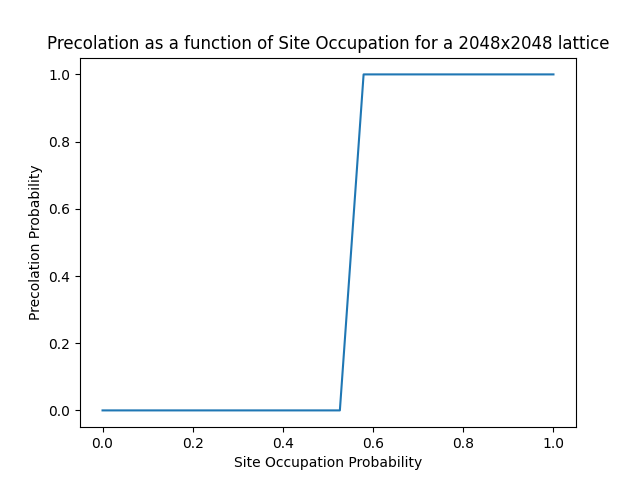
\includegraphics[width=0.5\textwidth]{images/q1.png}
    \caption{The graph of percolation probability as a function of cite occupation probability can be seen in figure \ref{fig:q1}. As can be seen, the precolation probability jumps sharply around $p = p_c = 0.618$, as expected for such a large lattice.}
    \label{fig:q1}
\end{figure}
\subsection{The critical cite occupation probability}
Around the critical cite occupation probability $p = p_c = 0.618$, we wanted to see how the lattice changes with coarse graining. To do this, we generated one lattice at $p = p_c$, one lattice at $p = 0.55$ and one lattice at $p = 0.65$. For each of these lattices, we repeatedly apploied coarse graining by a factor of 2, plotting the lattice itself and finally plotting the lattice occupation density as a function of the coarse graining iteration. The lattices can be seen in figures \ref{fig:lattices_55}, figure \ref{fig:lattices_pc}, and \ref{fig:lattices_65}, and the densitiy functions can be seen in figure \ref{fig:densities}.
\newline
As expected, the coarse graining operation for $p < p_c$ slowly decreases the lattice occupation density, while for $p > p_c$ is slowly increases it. for $p = p_c$, the density remains roughly the same. To see that it is actually constant, we generated four additional lattices at $p = p_c$, and plotted their average density for each coarse graining iteration. The result can be seen in figure \ref{fig:average_densities}. It is clear that the density at $p = p_c$ is invariant under the coarse graining operation.
\begin{figure}[h]
    \centering
    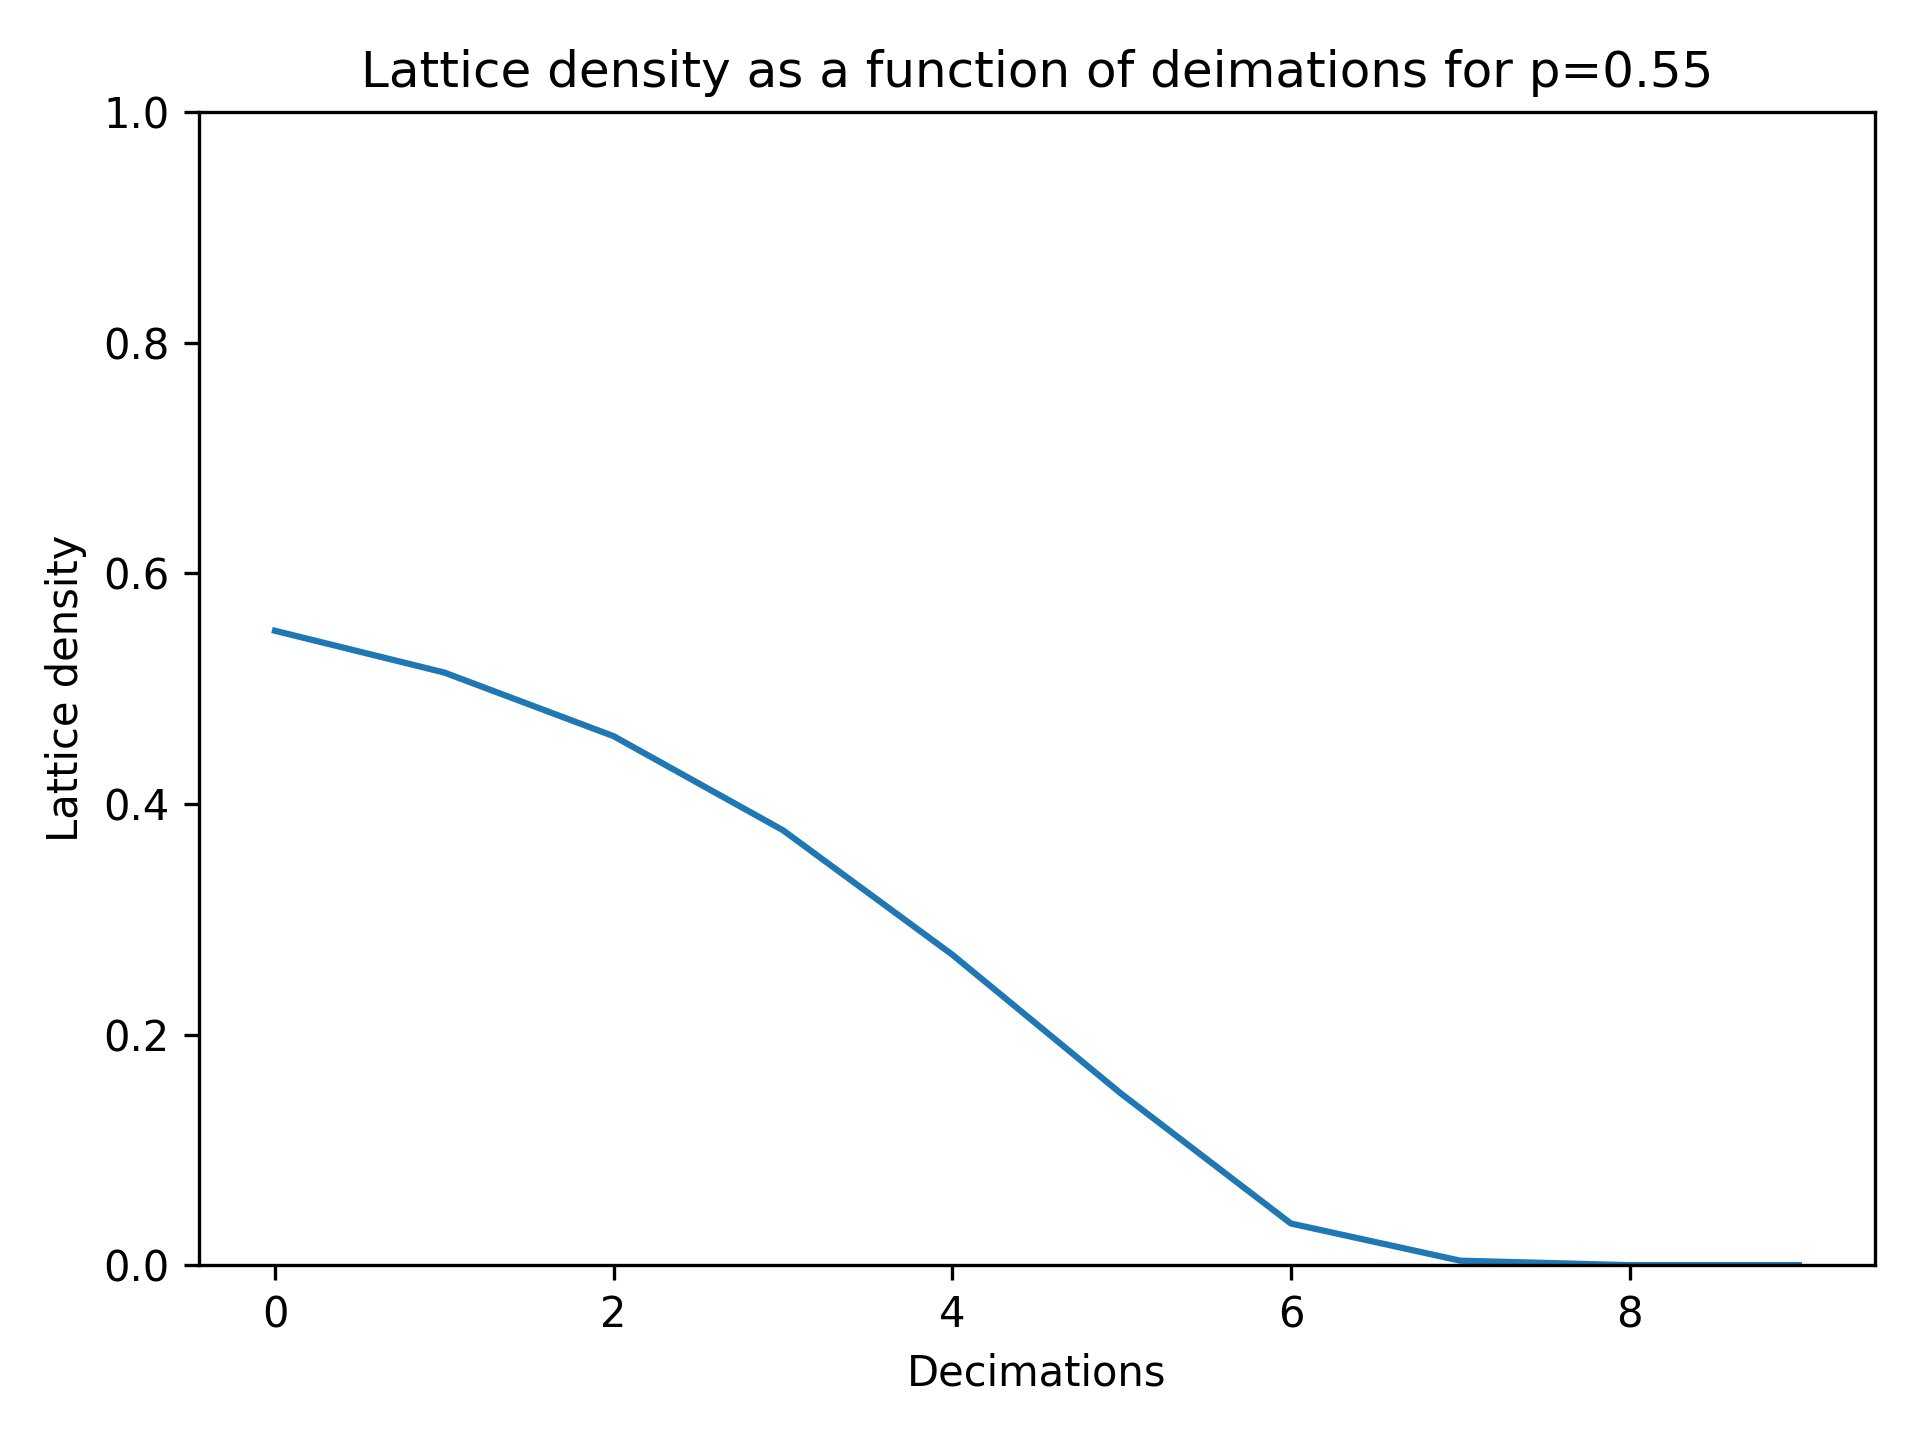
\includegraphics[width=0.3\textwidth]{images/Lattice density as a function of deimations for p=0.55.png}
    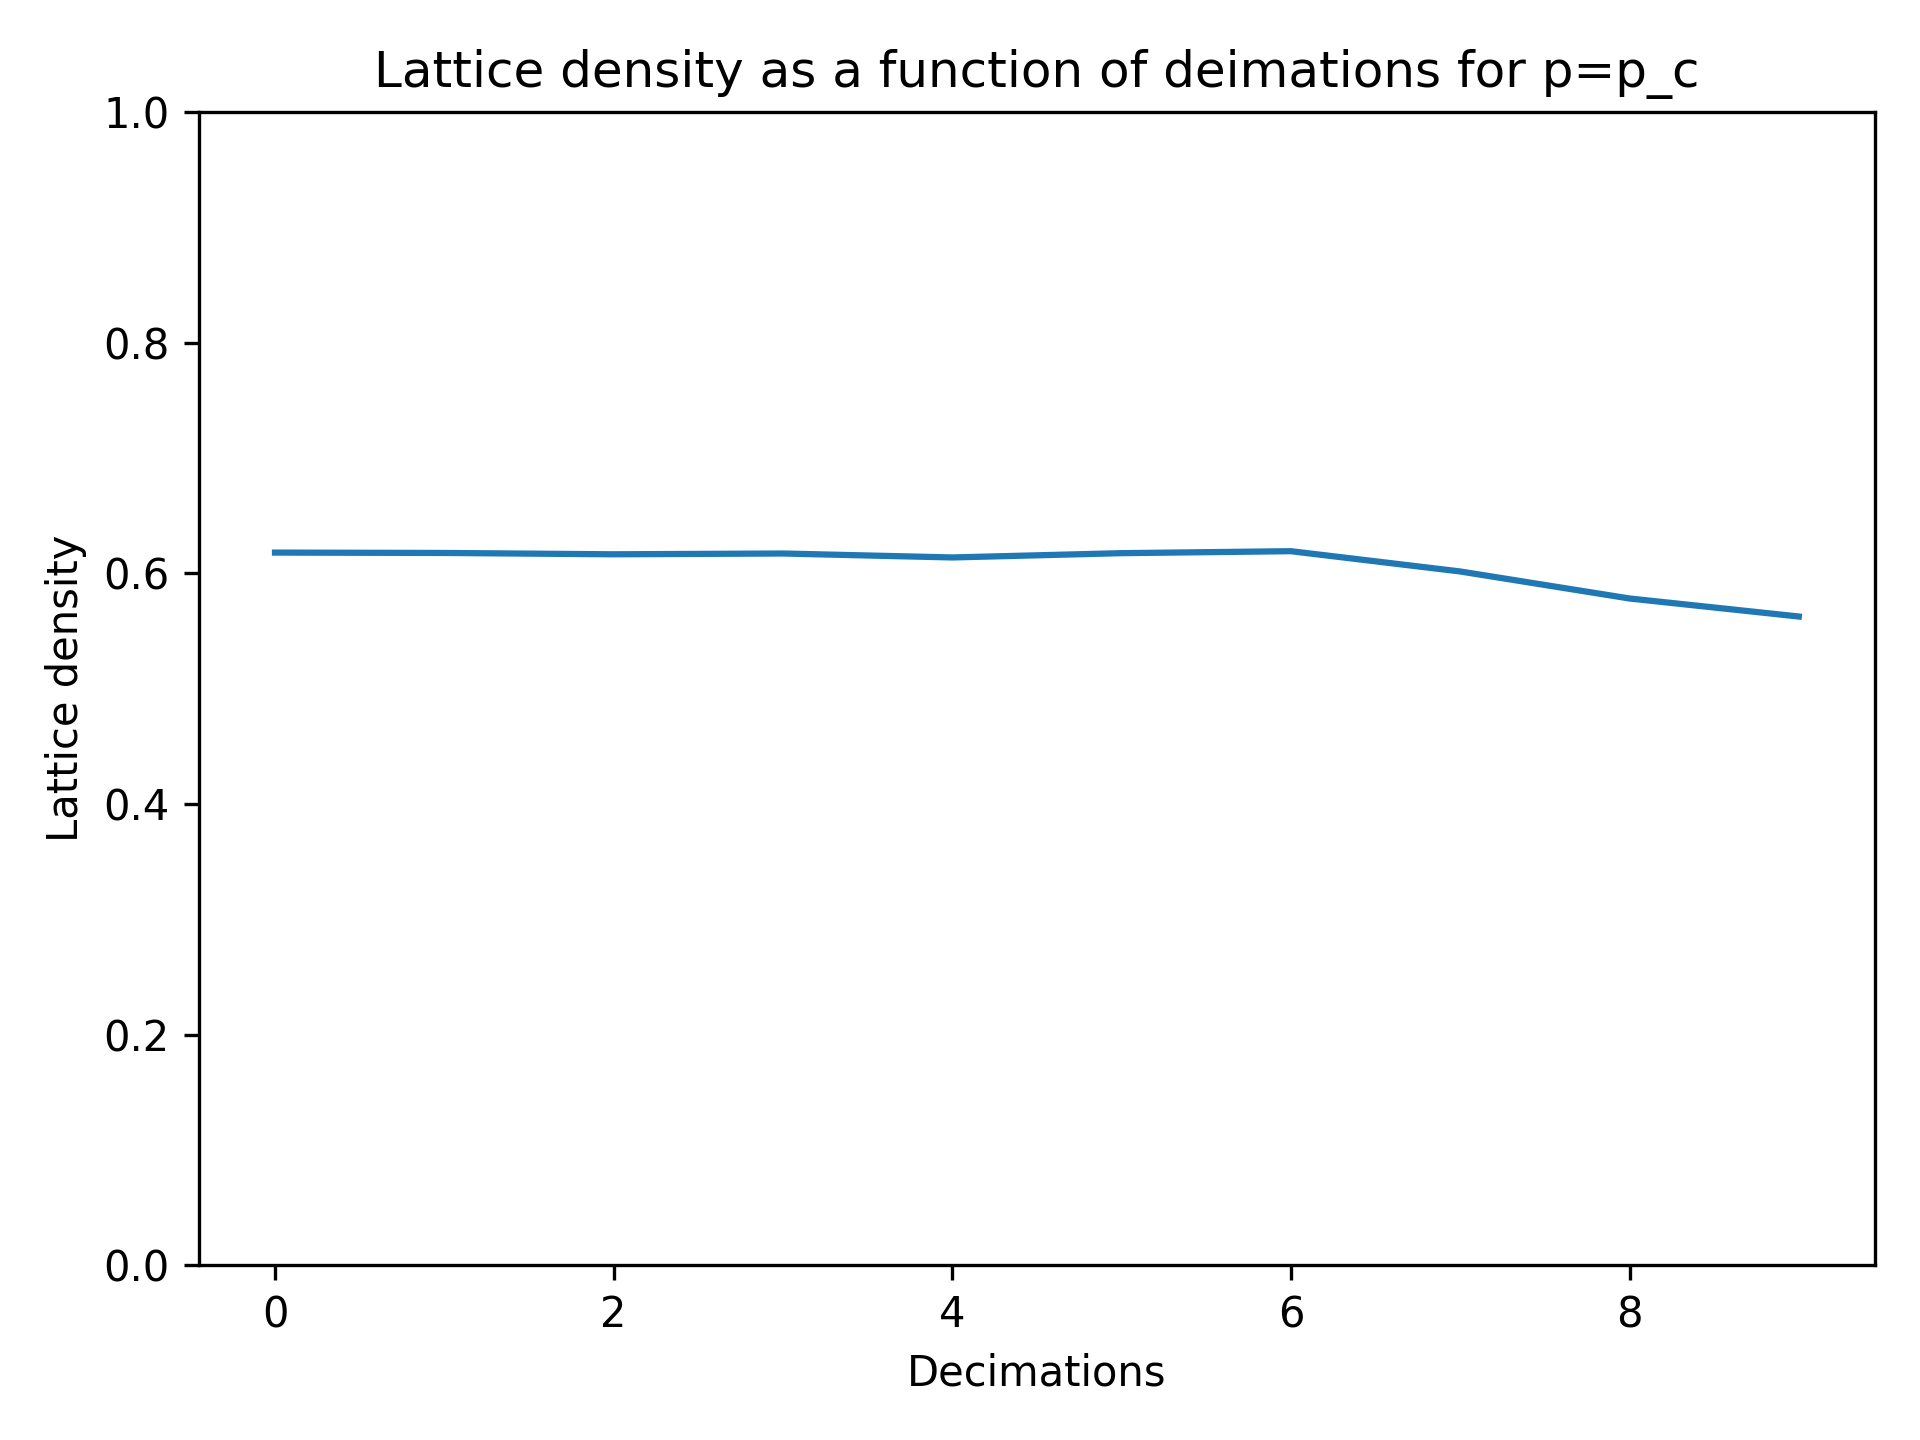
\includegraphics[width=0.3\textwidth]{images/Lattice density as a function of deimations for p=p_c.png}
    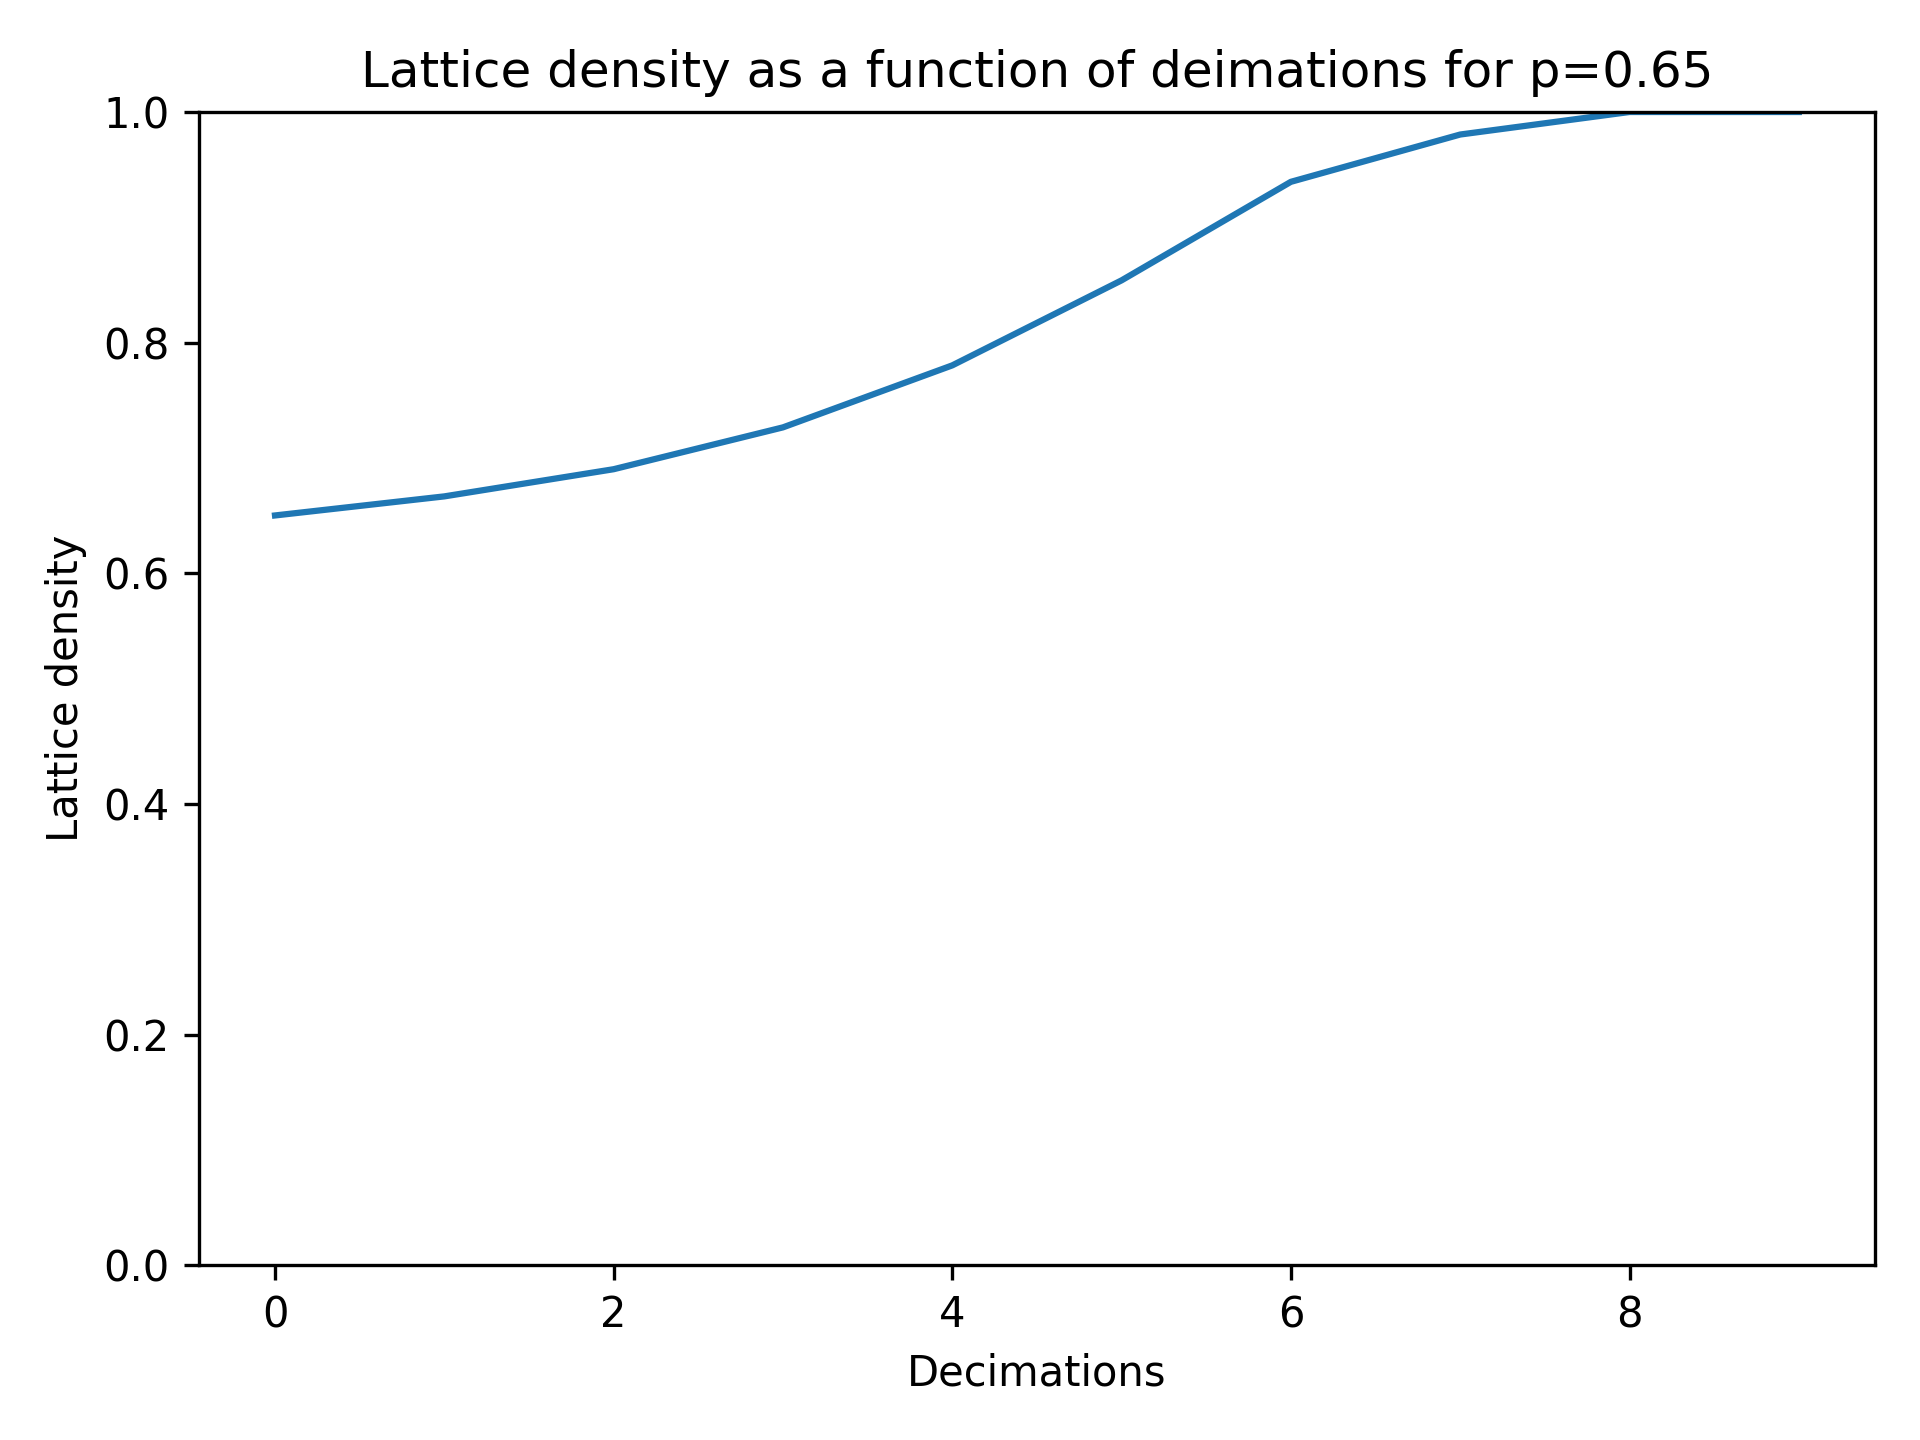
\includegraphics[width=0.3\textwidth]{images/Lattice density as a function of deimations for p=0.65.png}
    \caption{Lattice densities as a function of coarse graining iteration, for cite occupation probabilities $p = 0.55$ (left), $p_c = 0.618$ (center), and $p = 0.65$ (right).}
    \label{fig:densities}
\end{figure}
\begin{figure}[h]
    \centering
    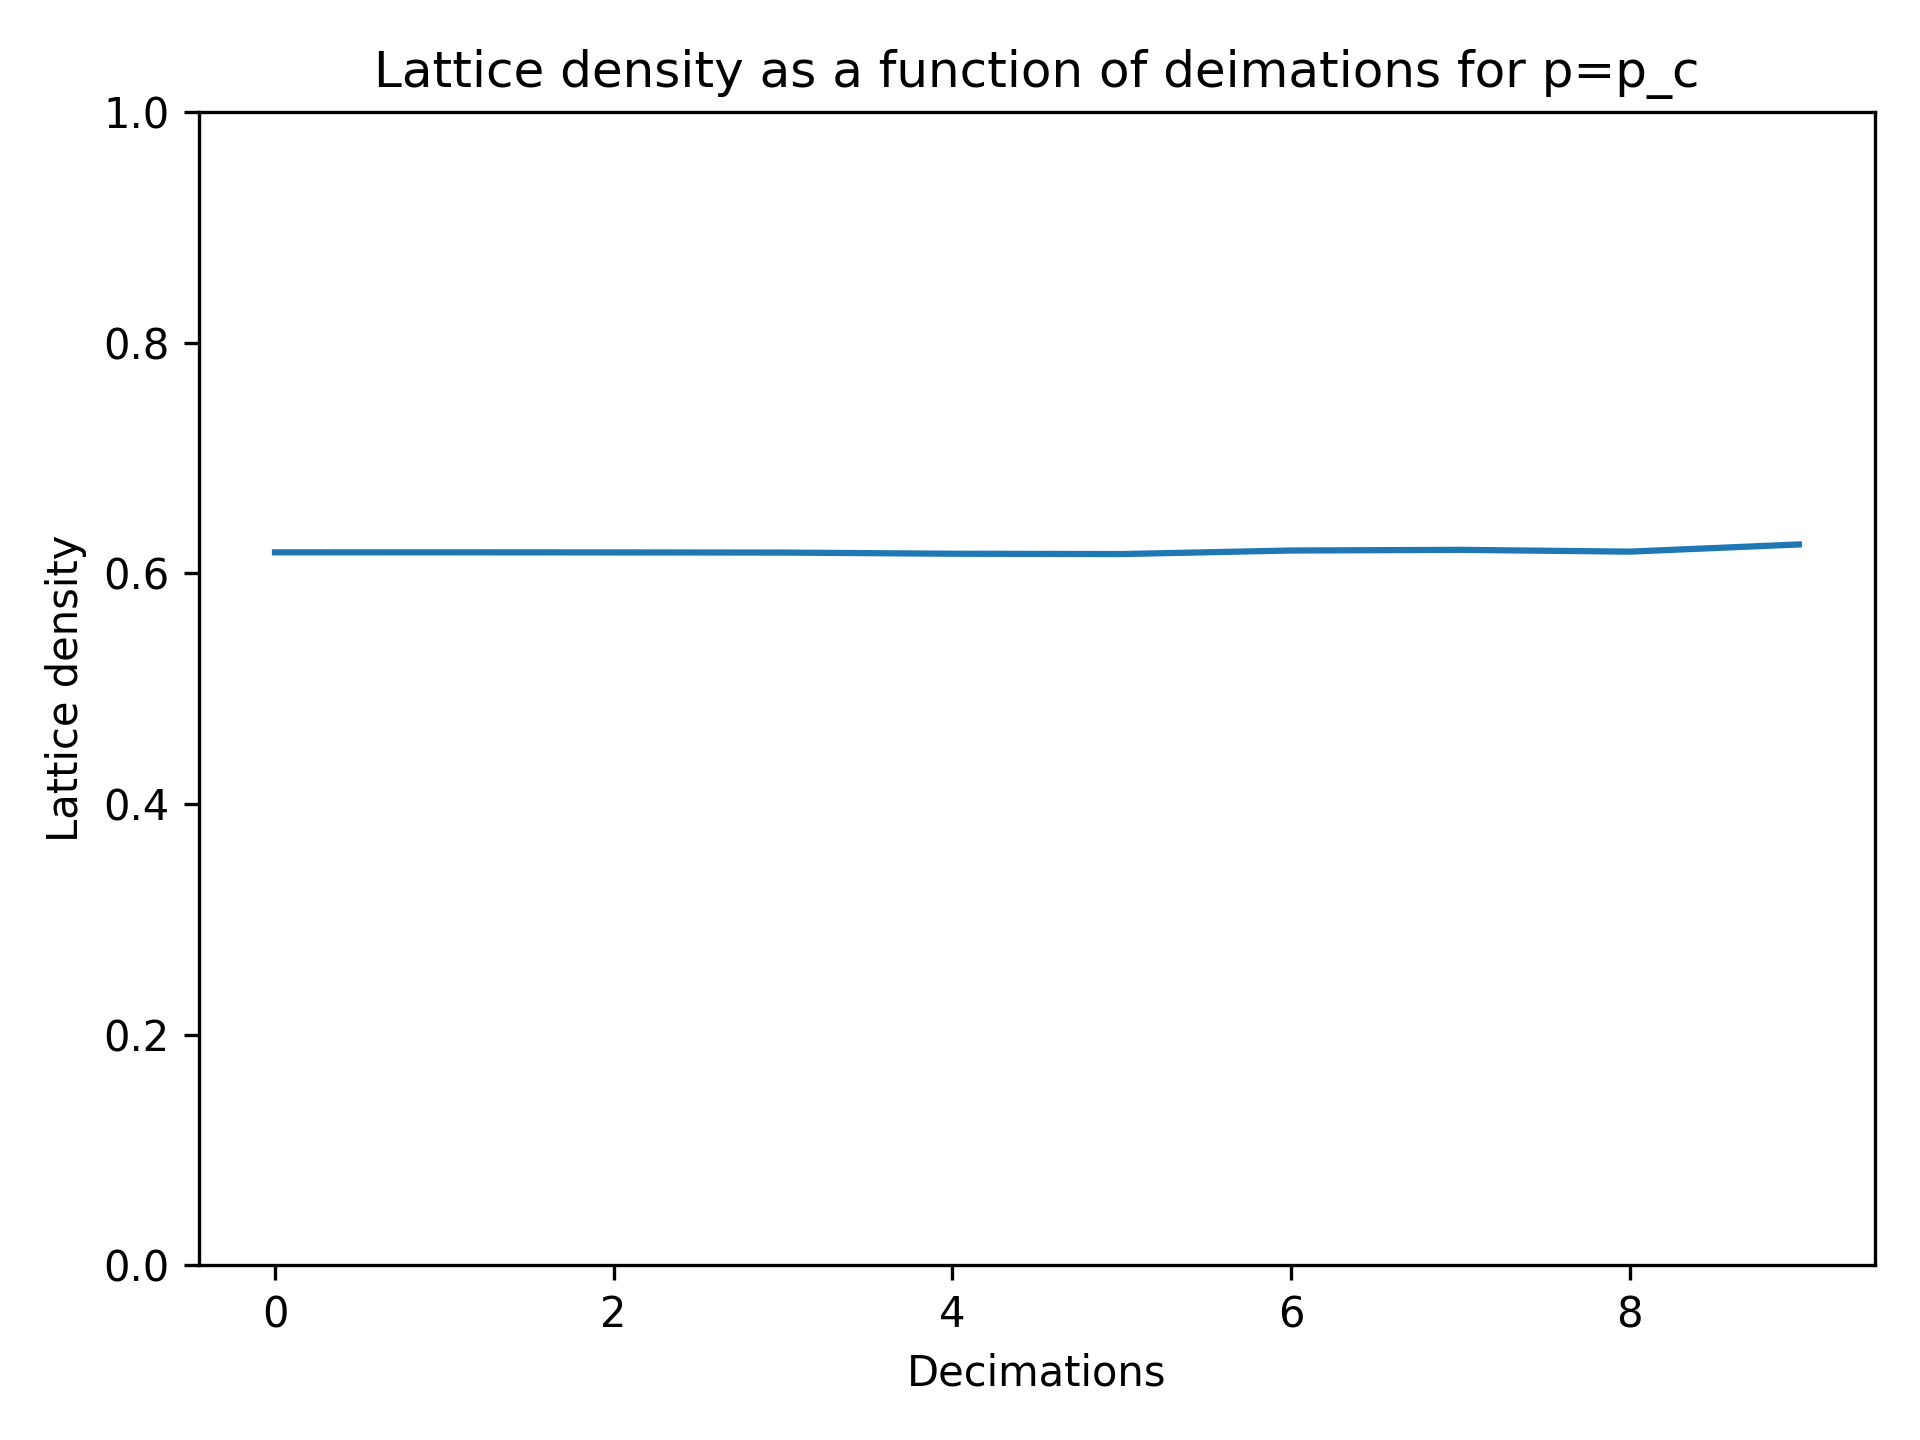
\includegraphics[width=0.5\textwidth]{images/Average lattice density as a function of deimations for p=p_c.png}
    \caption{Average lattice densities of five randomally generated lattices as a function of coarse graining iteration, for cite occupation probabilities $p = p_c$.}
    \label{fig:average_densities}
\end{figure}
\begin{figure}[h]
    \centering
    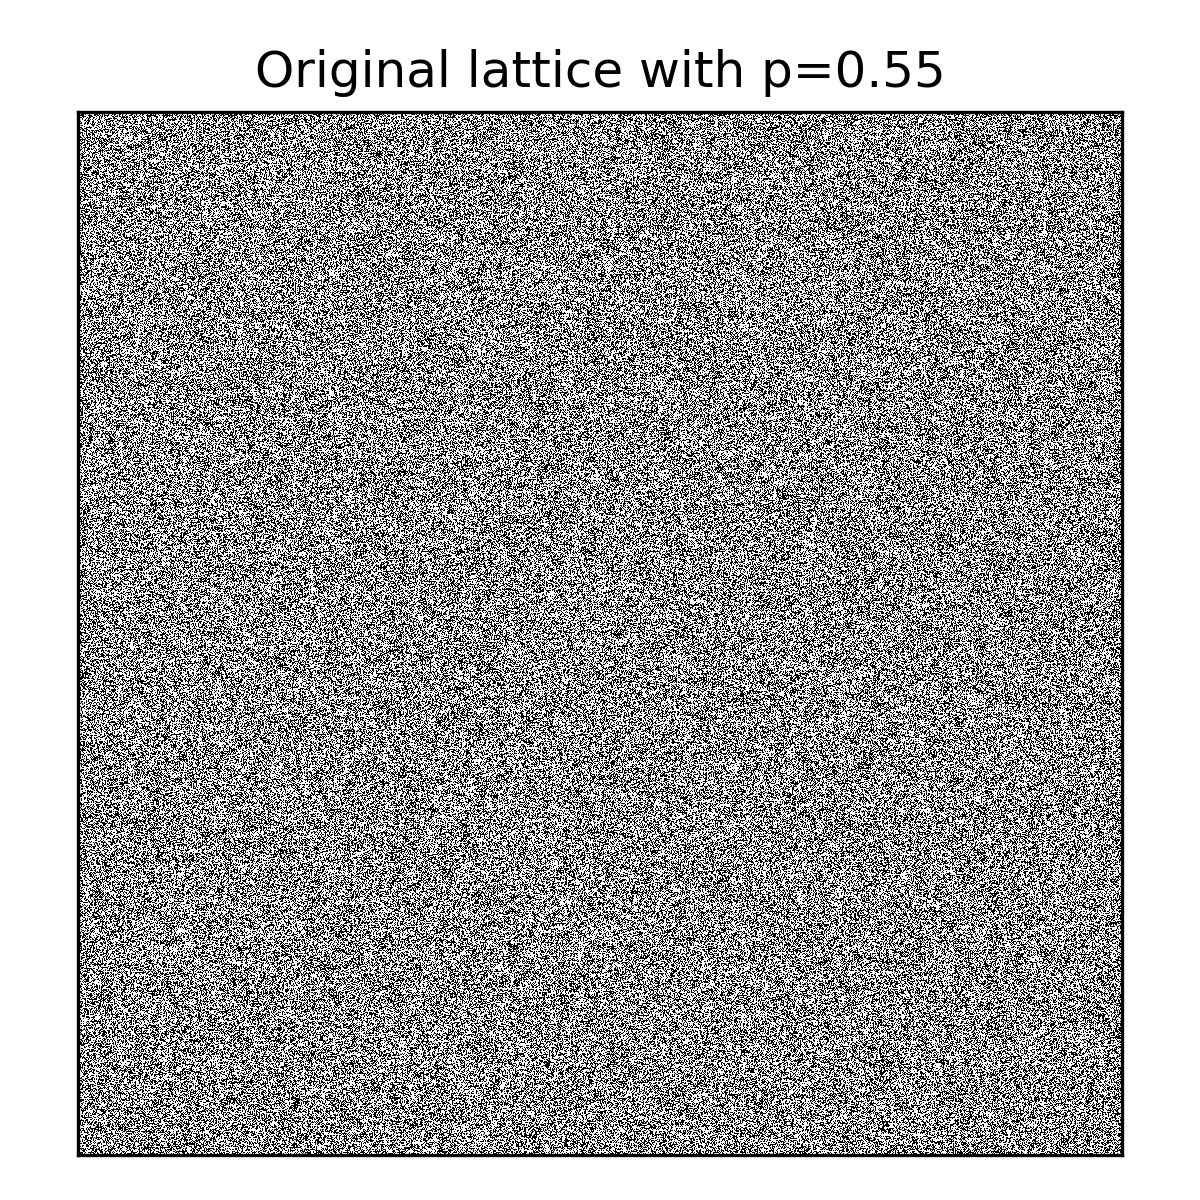
\includegraphics[width=0.3\textwidth]{images/Original lattice with p=0.55.png}
    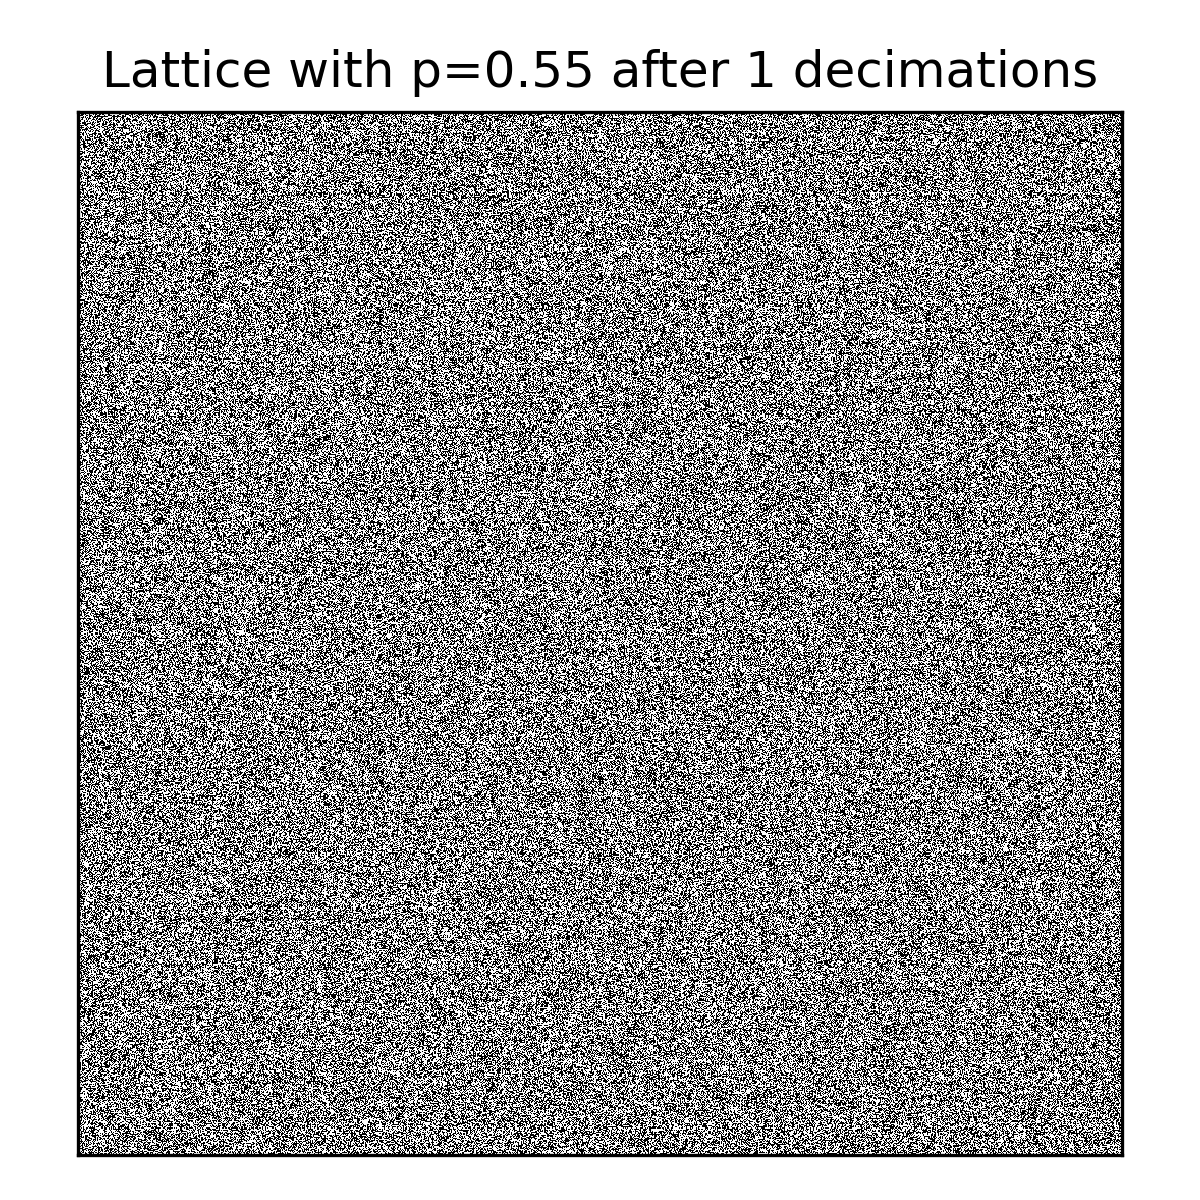
\includegraphics[width=0.3\textwidth]{images/Lattice with p=0.55 after 1 decimations.png}
    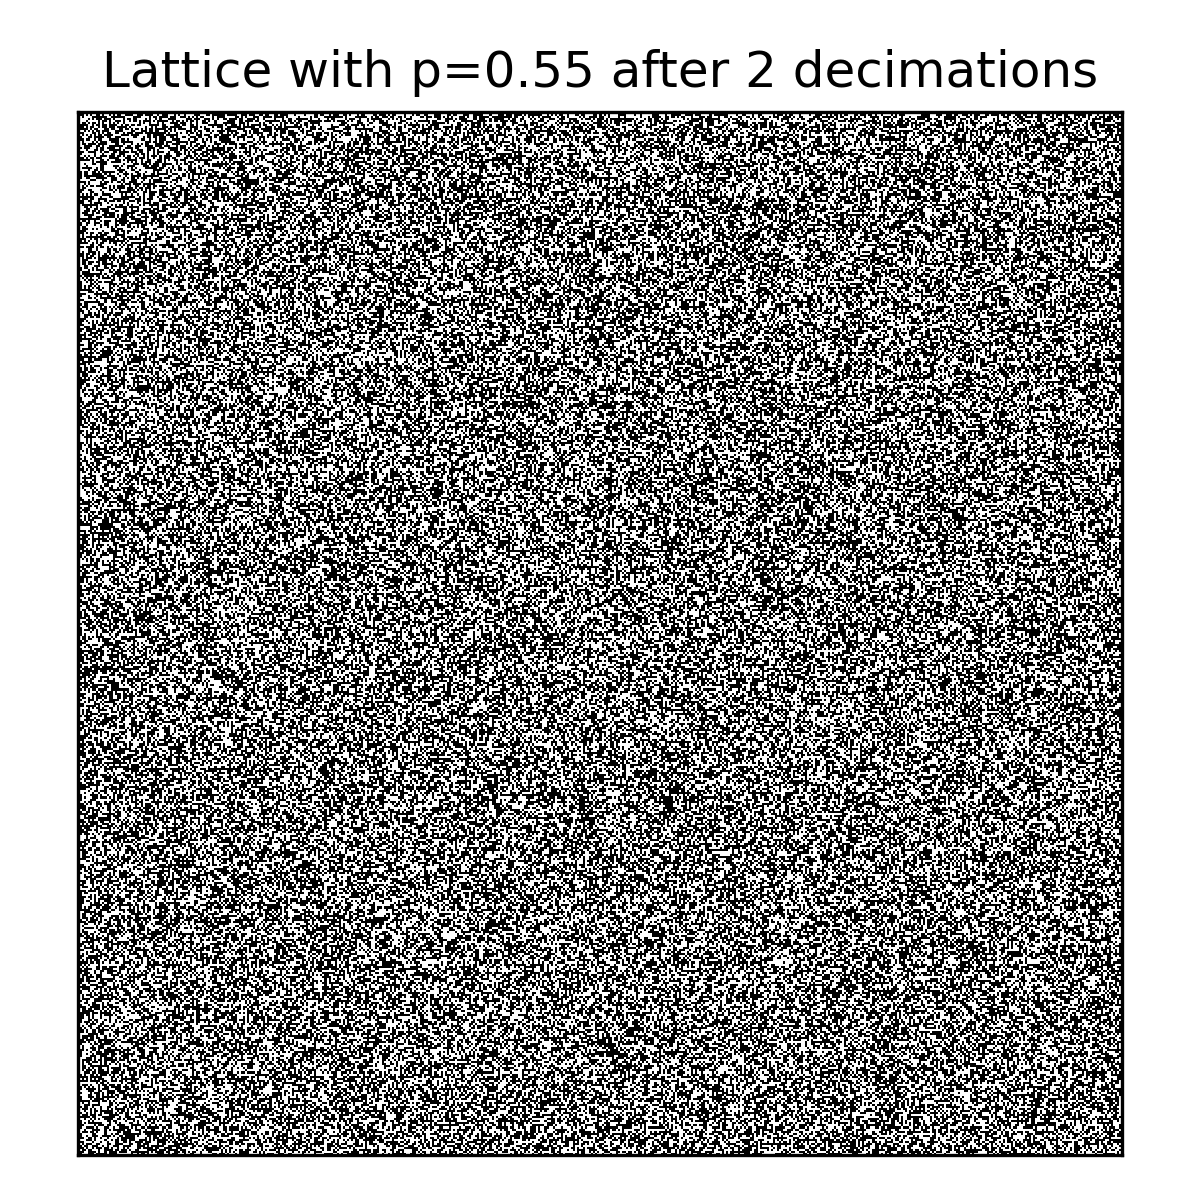
\includegraphics[width=0.3\textwidth]{images/Lattice with p=0.55 after 2 decimations.png}
    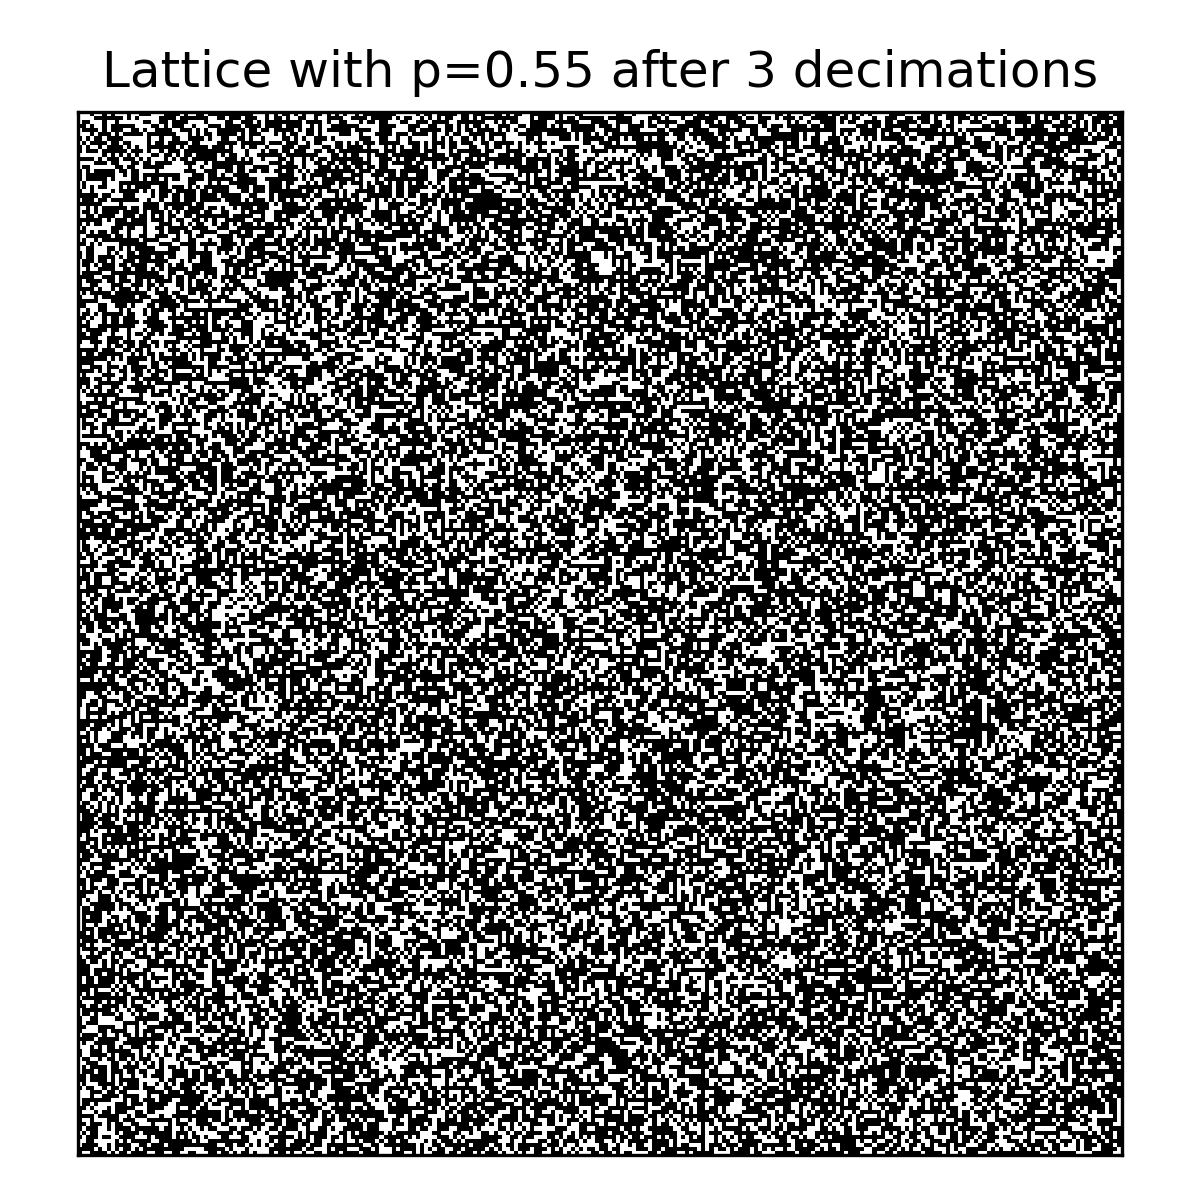
\includegraphics[width=0.3\textwidth]{images/Lattice with p=0.55 after 3 decimations.png}
    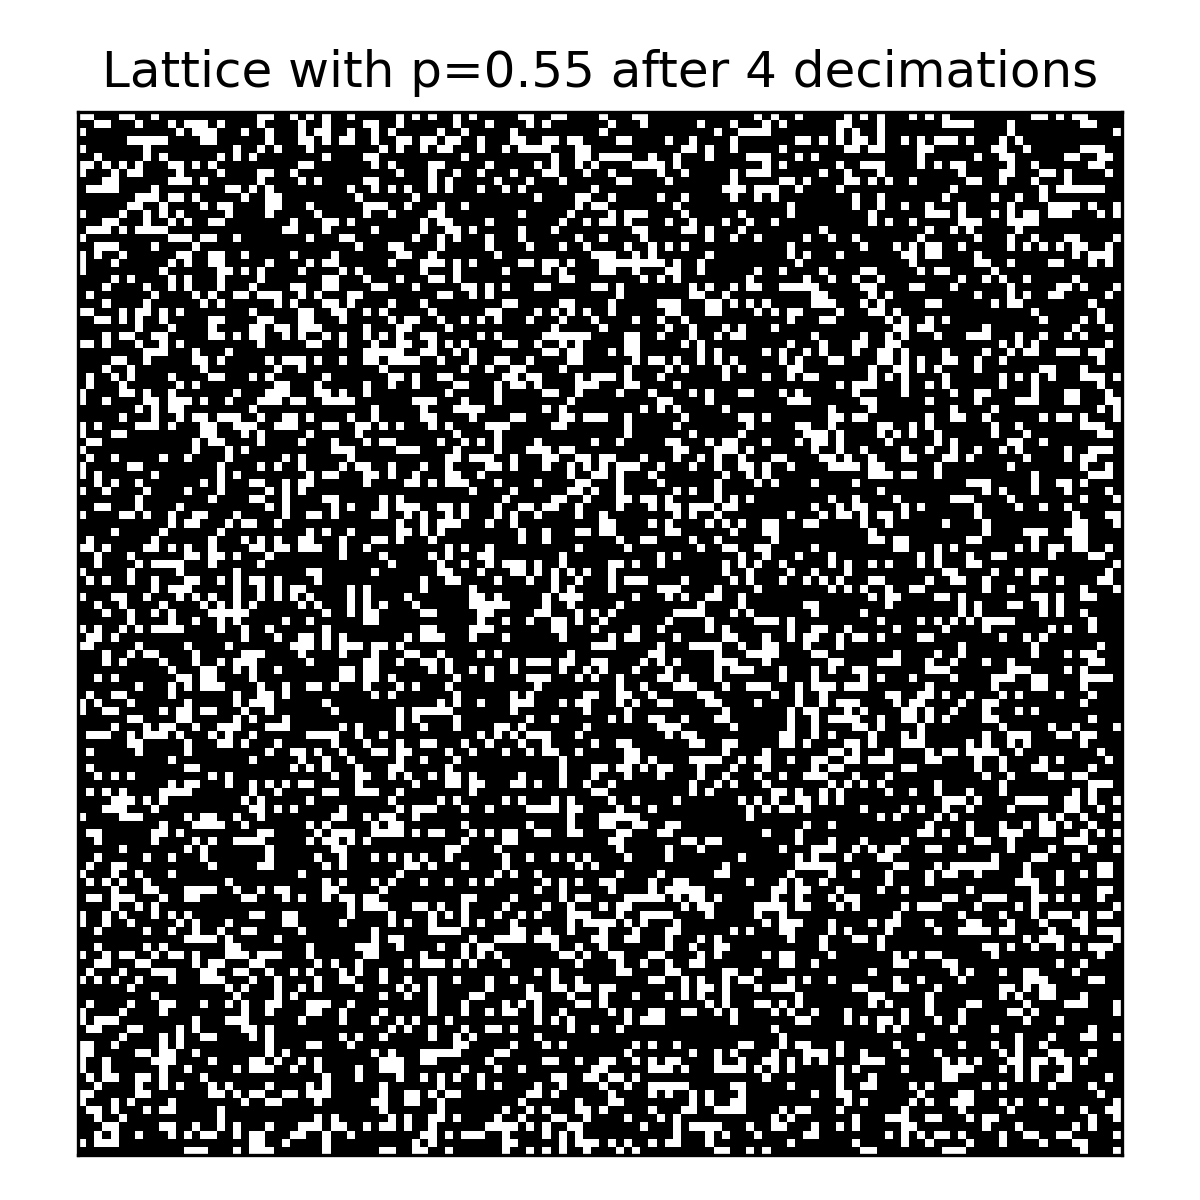
\includegraphics[width=0.3\textwidth]{images/Lattice with p=0.55 after 4 decimations.png}
    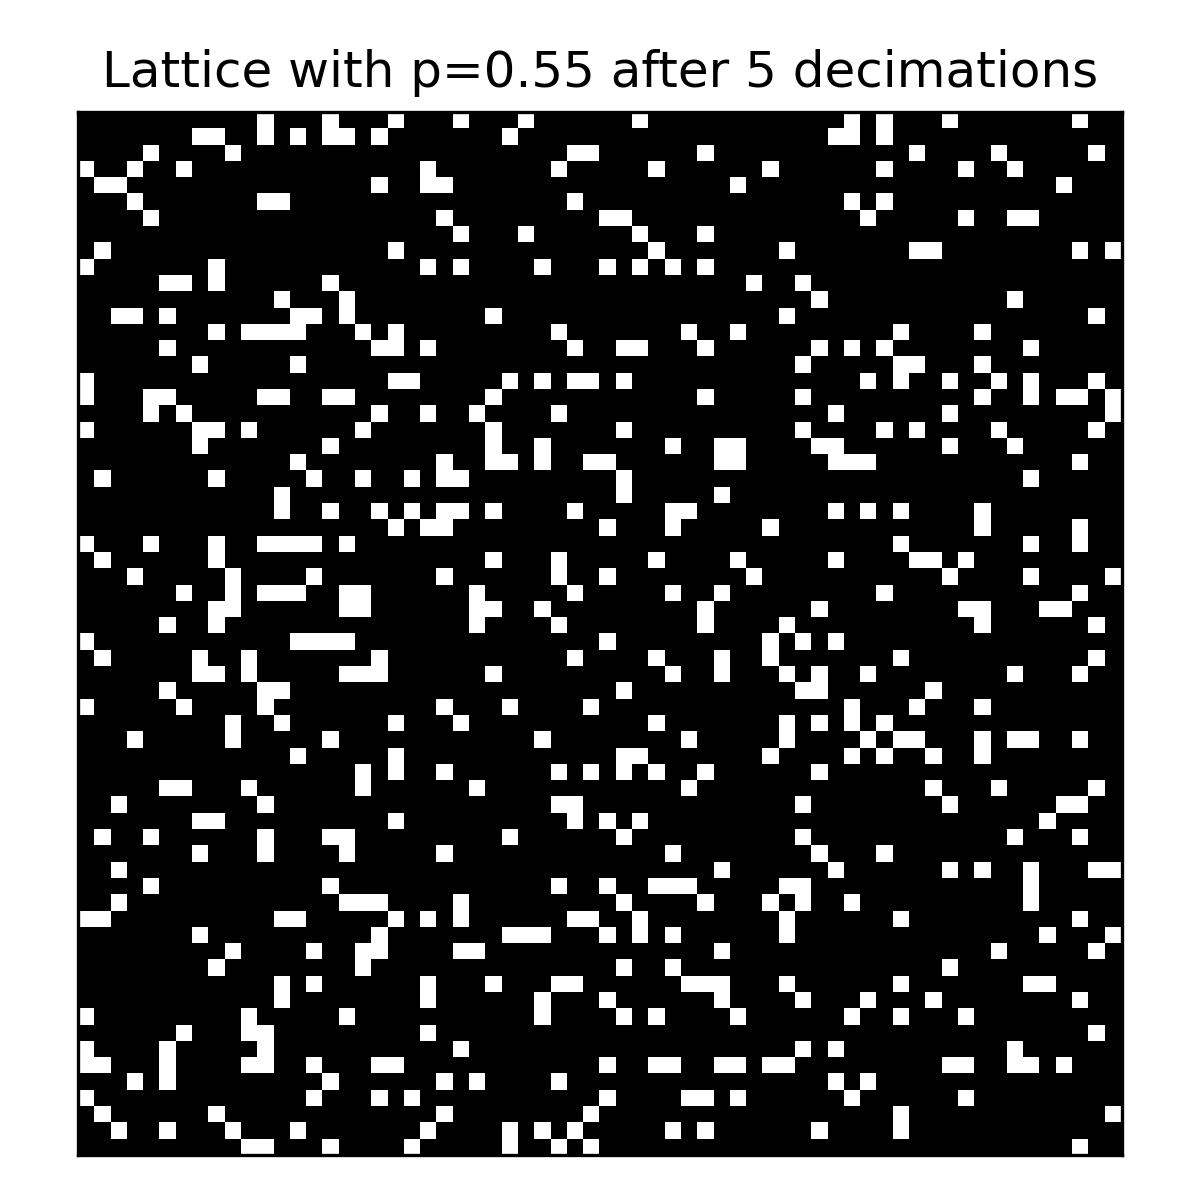
\includegraphics[width=0.3\textwidth]{images/Lattice with p=0.55 after 5 decimations.png}
    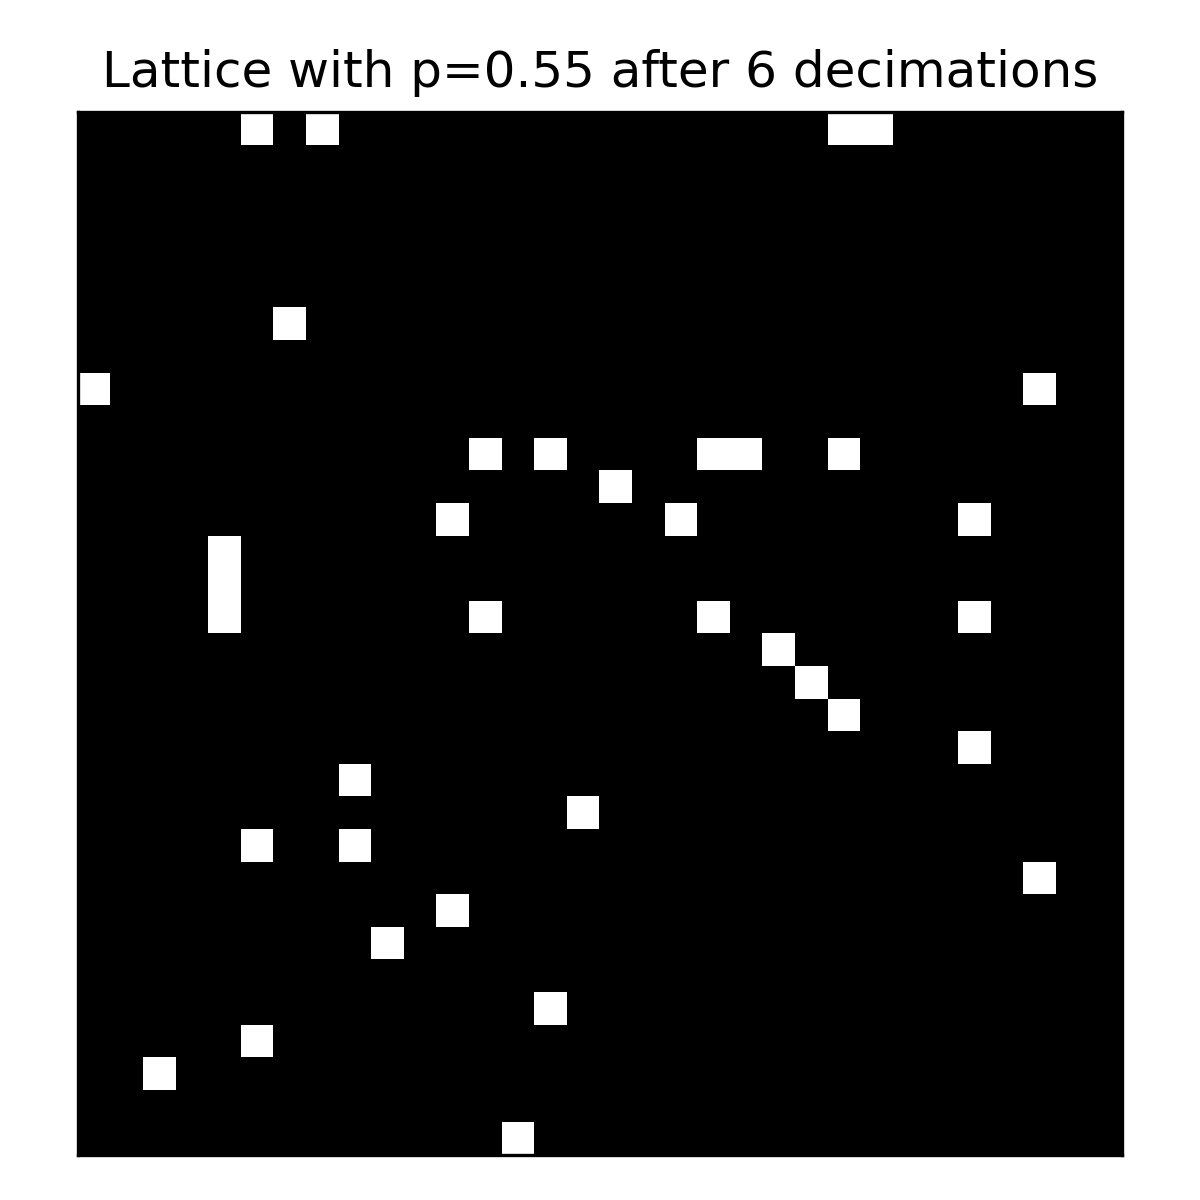
\includegraphics[width=0.3\textwidth]{images/Lattice with p=0.55 after 6 decimations.png}
    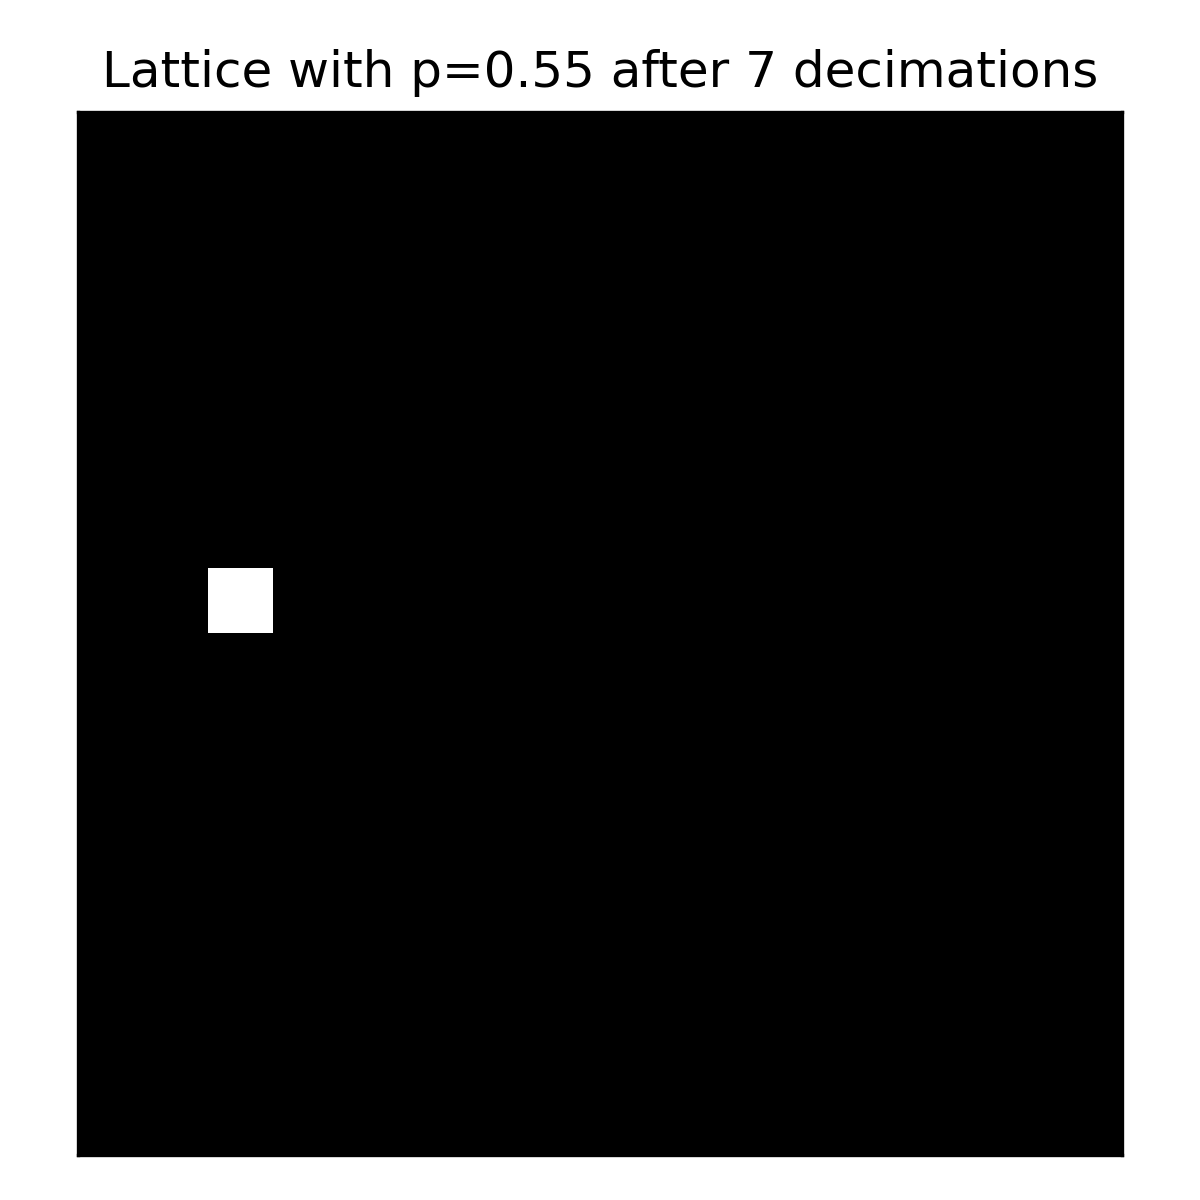
\includegraphics[width=0.3\textwidth]{images/Lattice with p=0.55 after 7 decimations.png}
    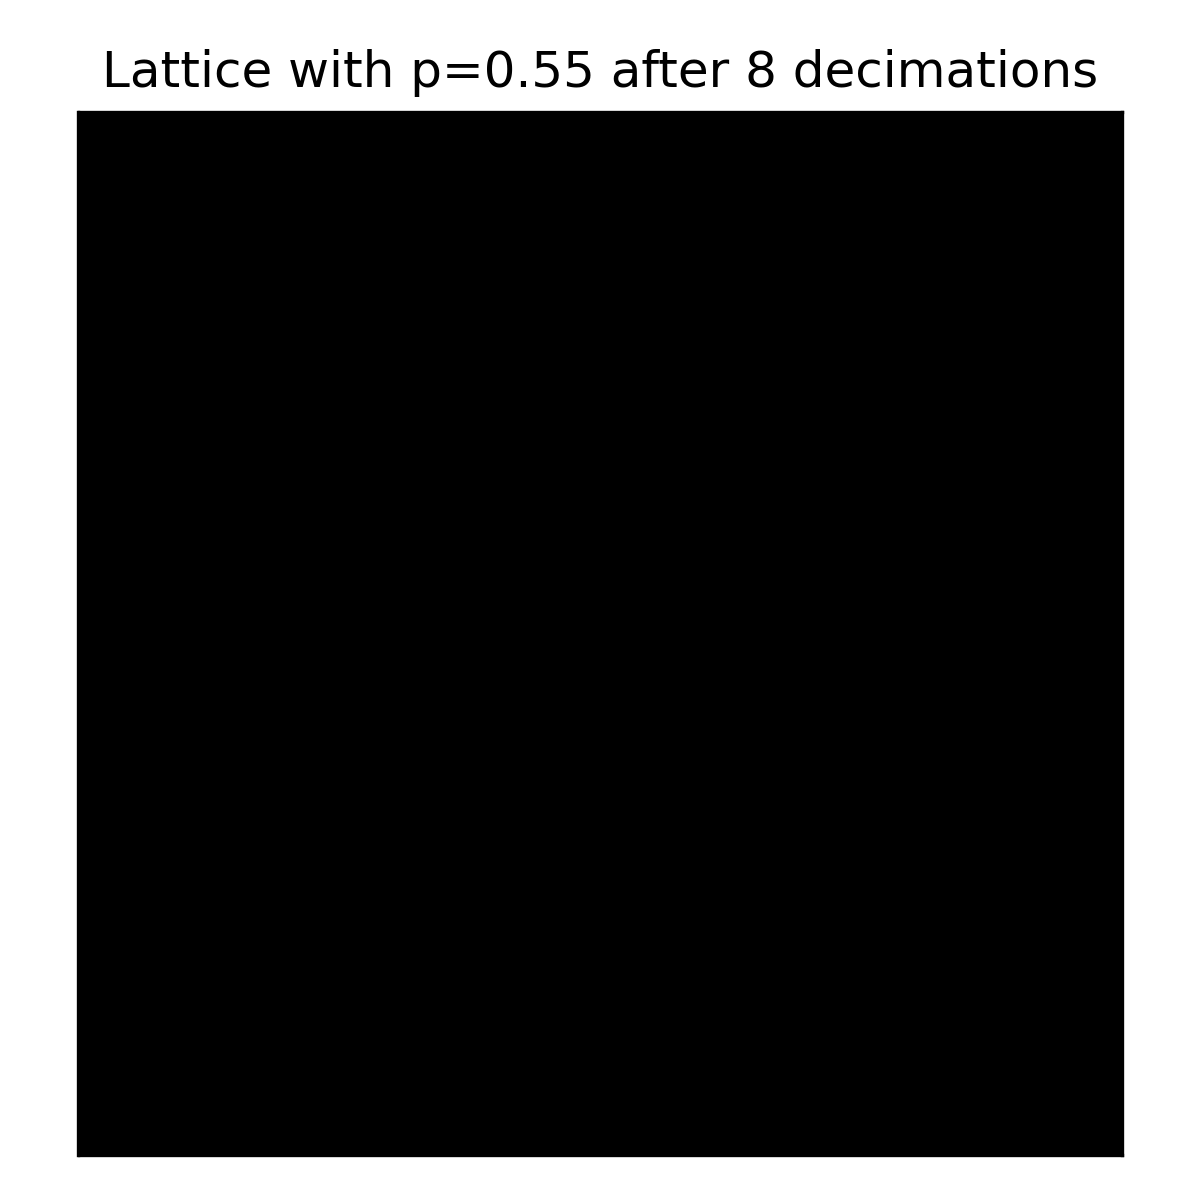
\includegraphics[width=0.3\textwidth]{images/Lattice with p=0.55 after 8 decimations.png}
    \caption{A lattice with $p=0.55$ in different stages of the coarse graining. Occupied cites are white.}
    \label{fig:lattices_55}
\end{figure}
\begin{figure}[h]
    \centering
    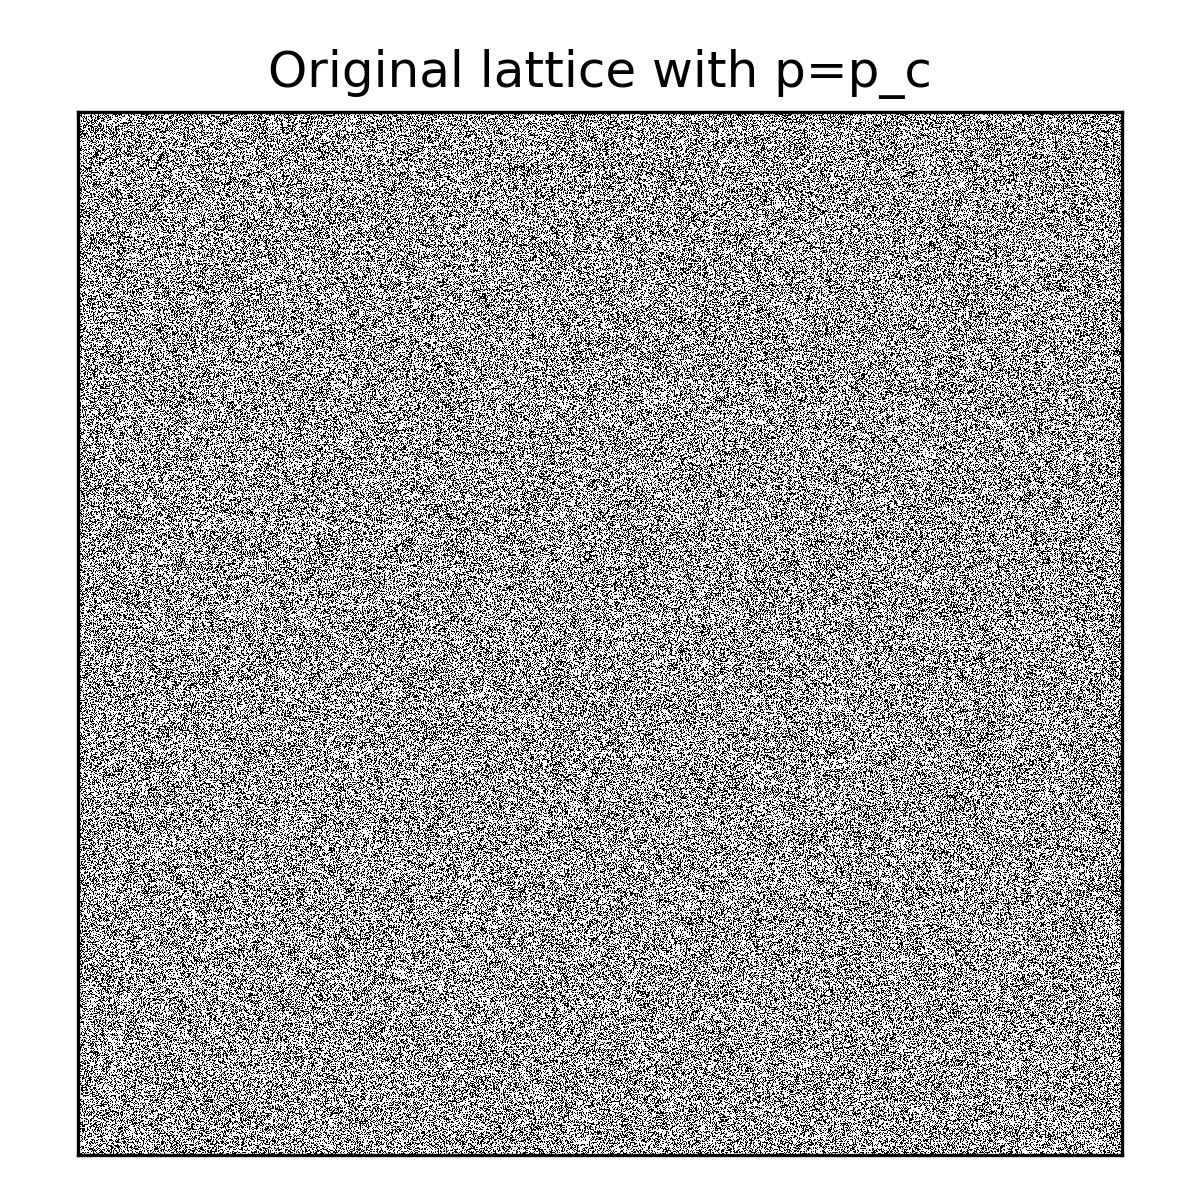
\includegraphics[width=0.3\textwidth]{images/Original lattice with p=p_c.png}
    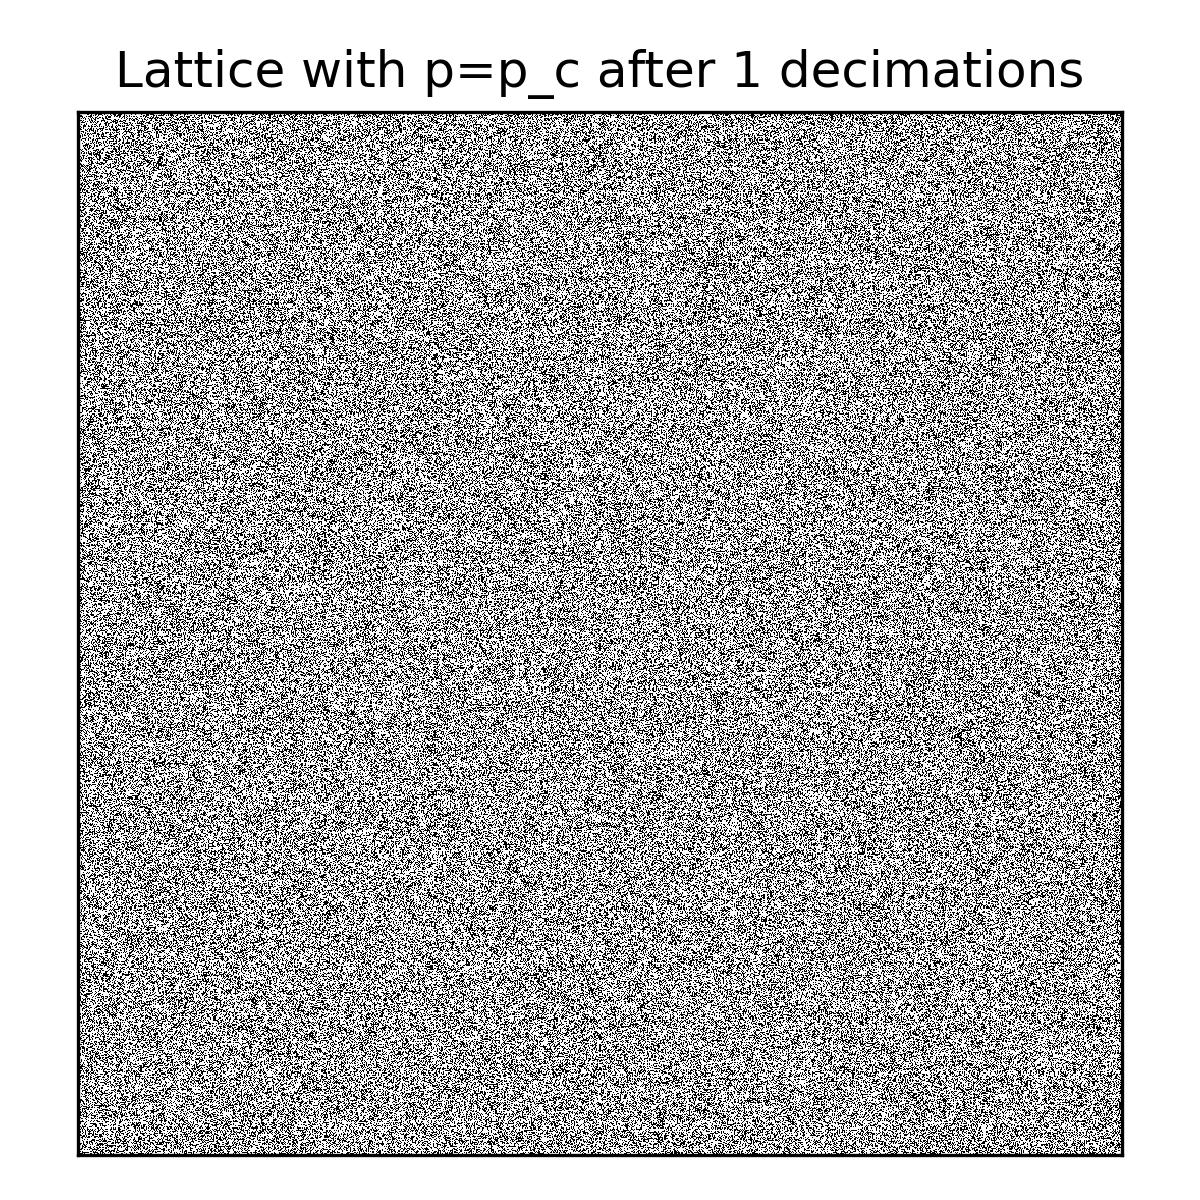
\includegraphics[width=0.3\textwidth]{images/Lattice with p=p_c after 1 decimations.png}
    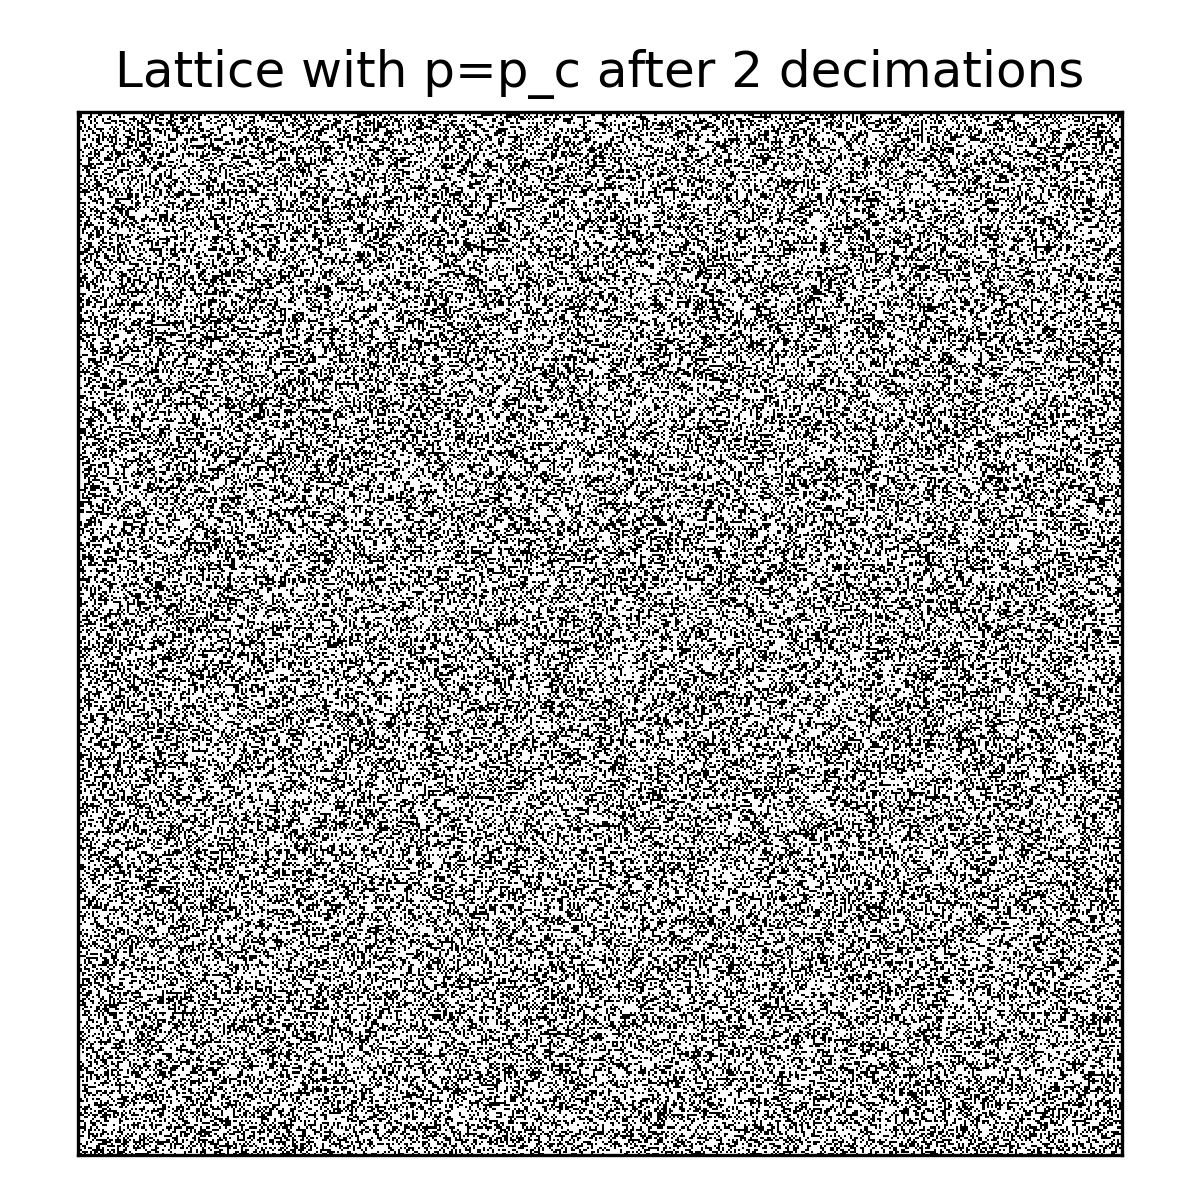
\includegraphics[width=0.3\textwidth]{images/Lattice with p=p_c after 2 decimations.png}
    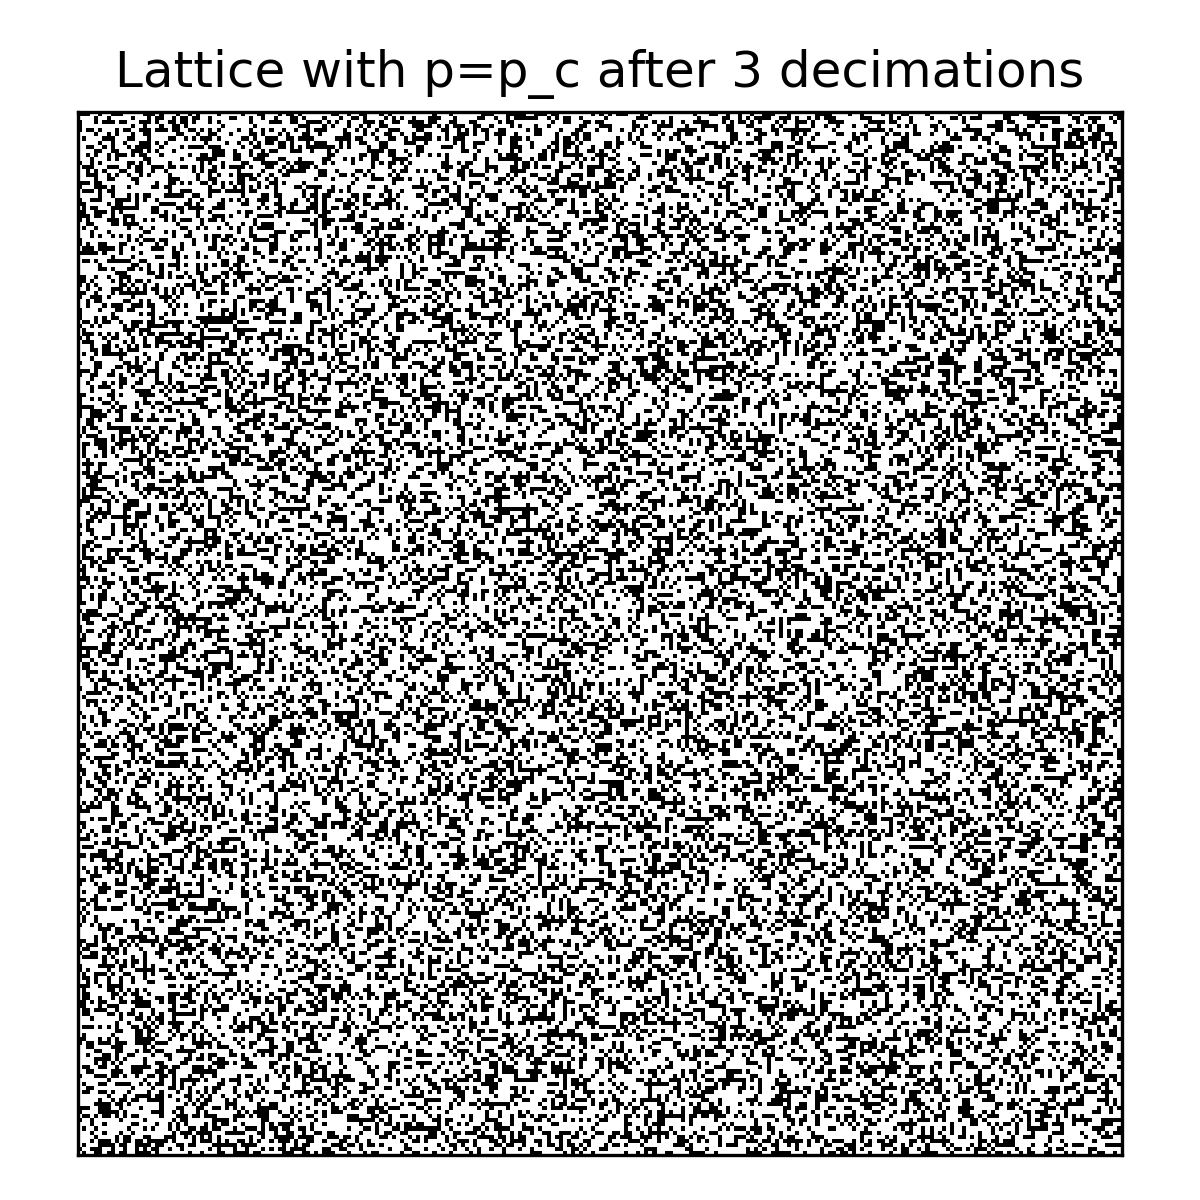
\includegraphics[width=0.3\textwidth]{images/Lattice with p=p_c after 3 decimations.png}
    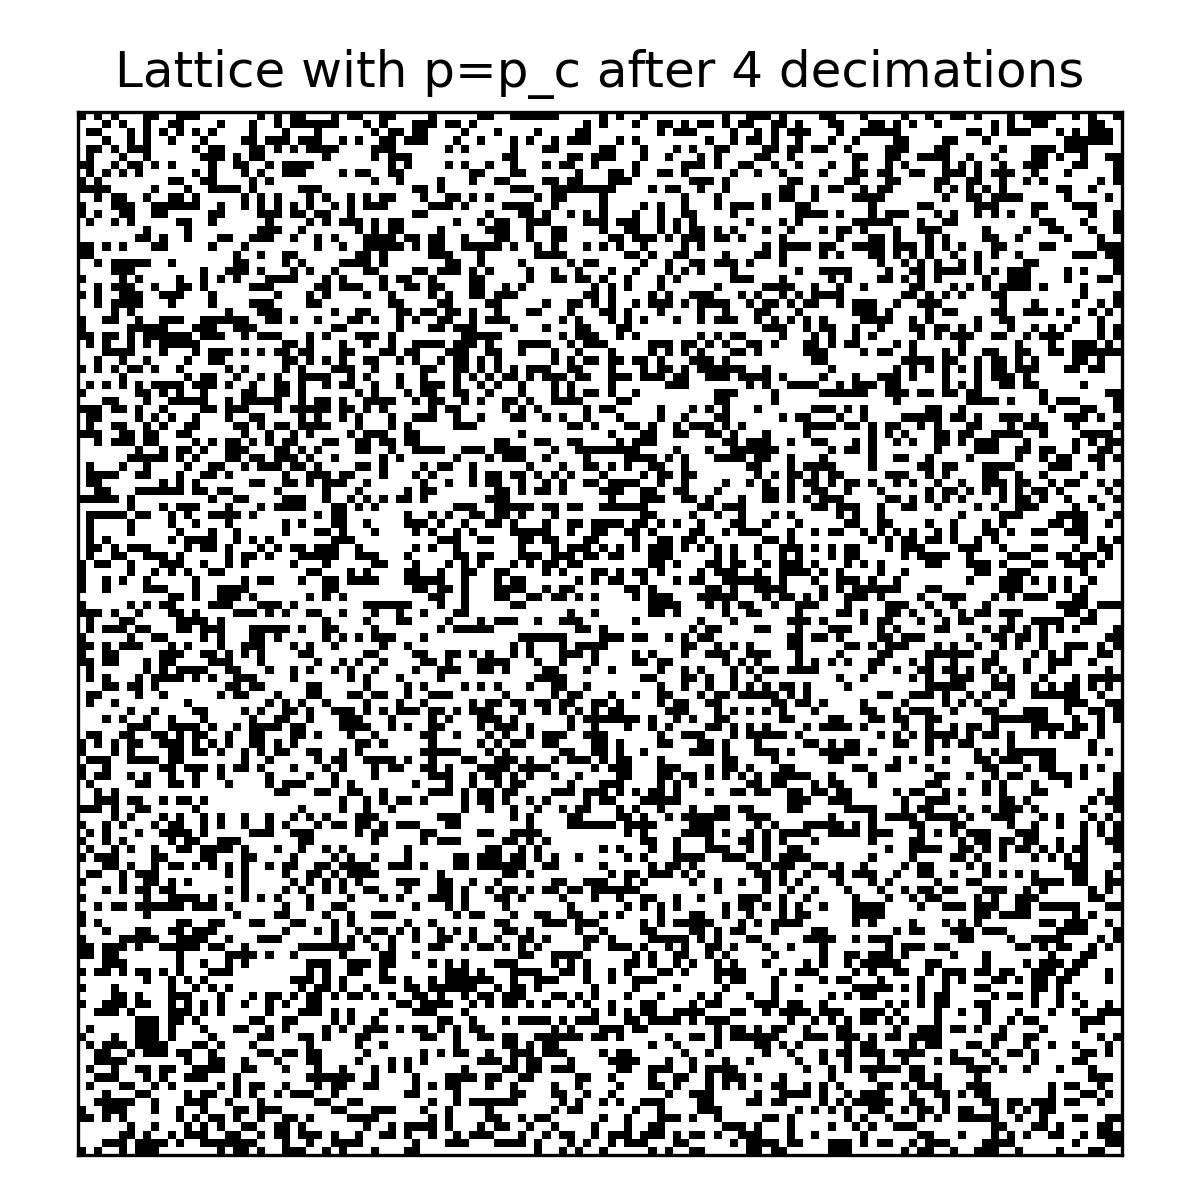
\includegraphics[width=0.3\textwidth]{images/Lattice with p=p_c after 4 decimations.png}
    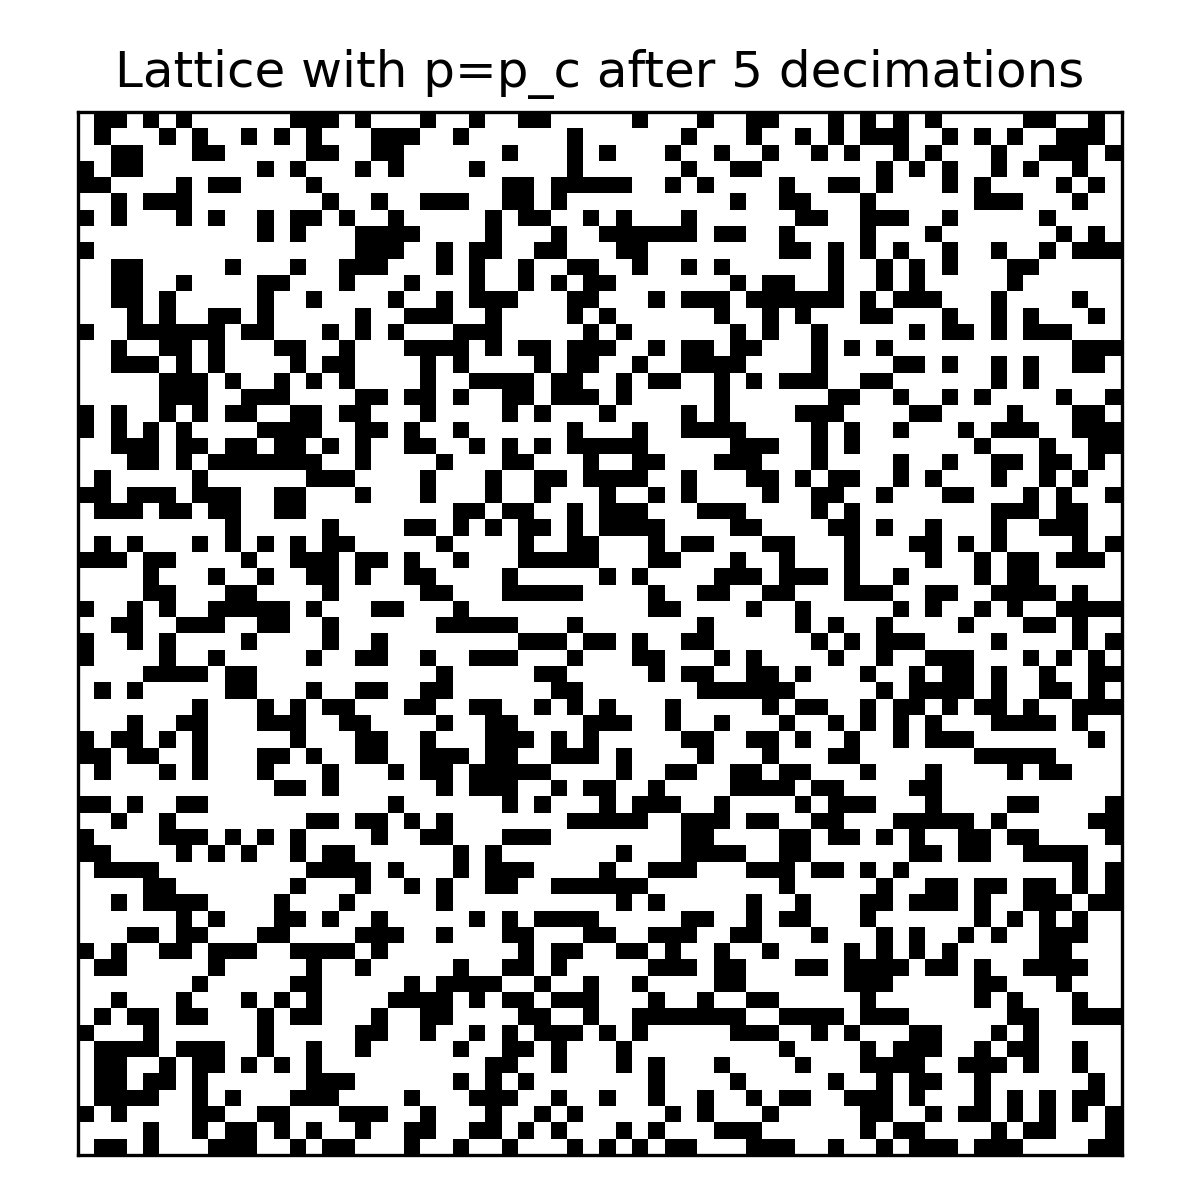
\includegraphics[width=0.3\textwidth]{images/Lattice with p=p_c after 5 decimations.png}
    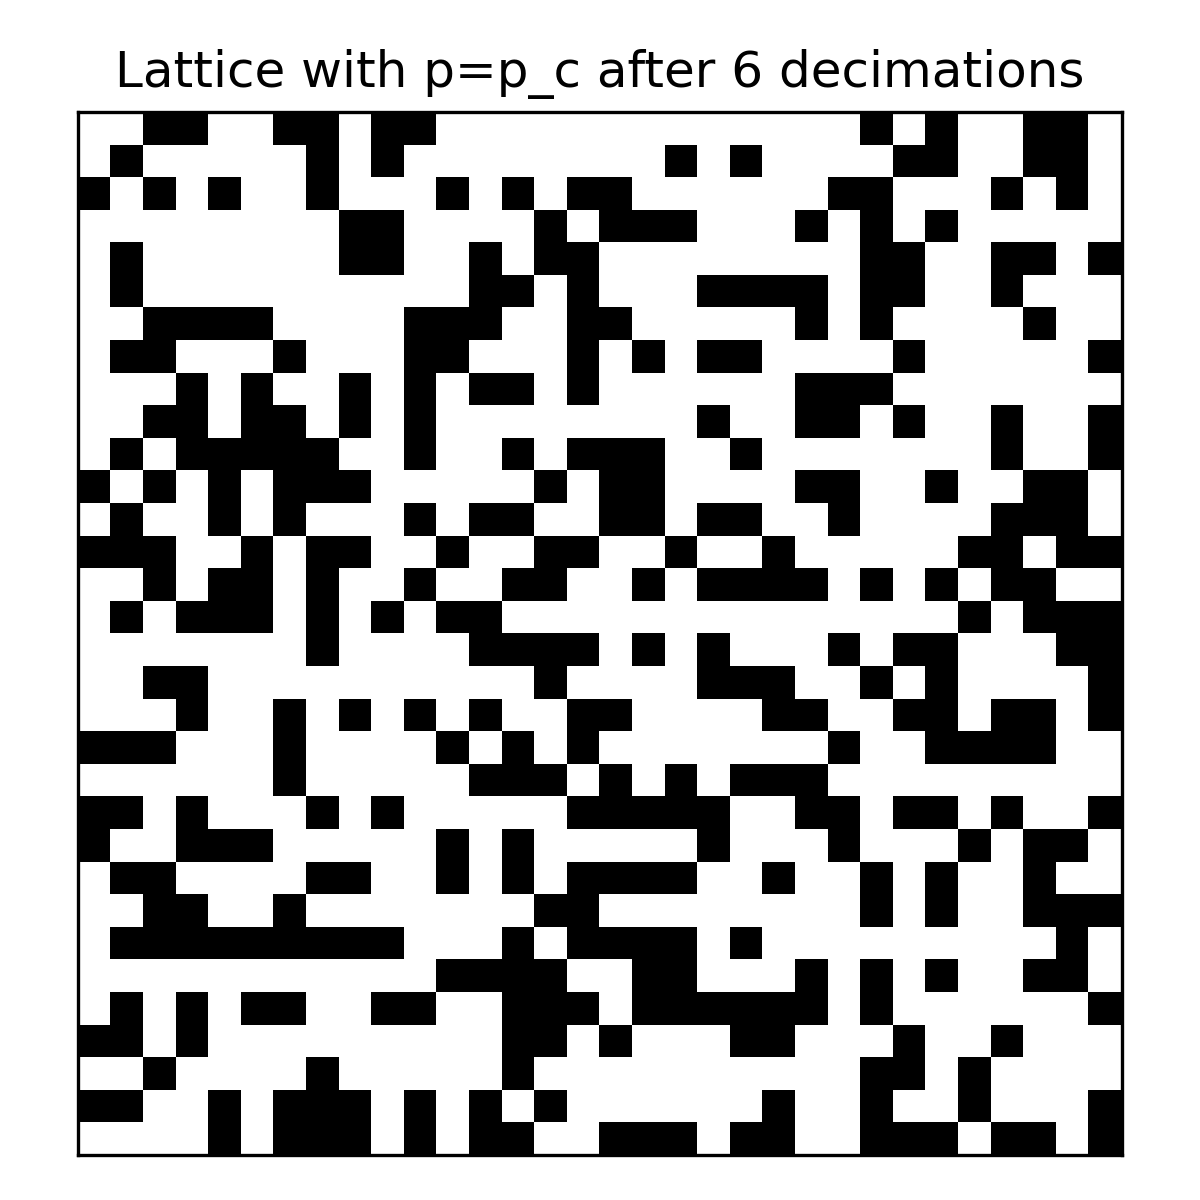
\includegraphics[width=0.3\textwidth]{images/Lattice with p=p_c after 6 decimations.png}
    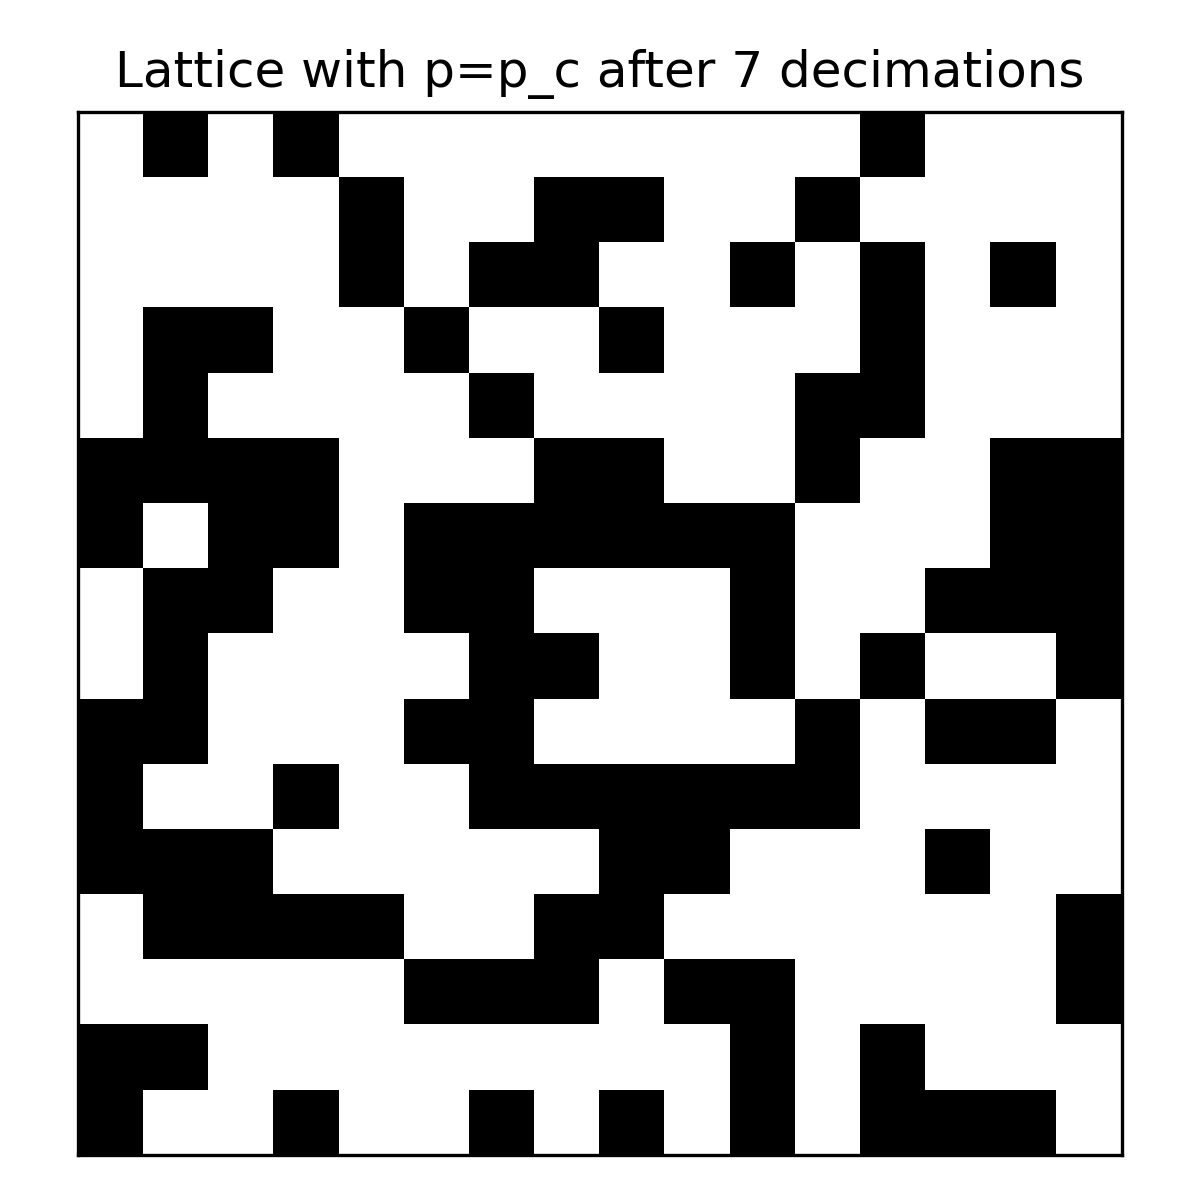
\includegraphics[width=0.3\textwidth]{images/Lattice with p=p_c after 7 decimations.png}
    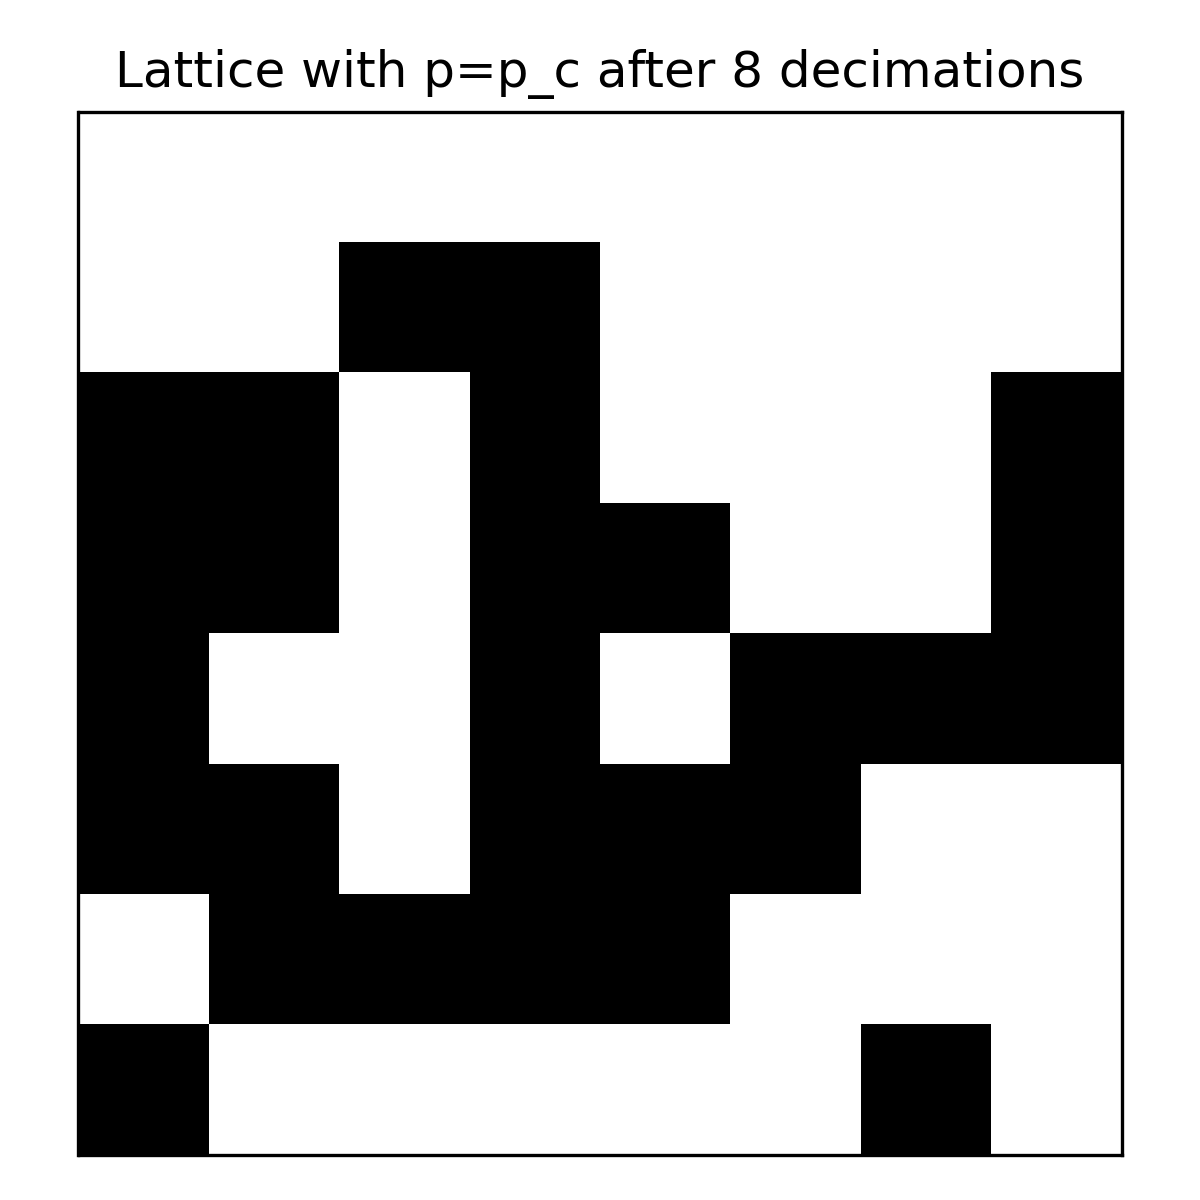
\includegraphics[width=0.3\textwidth]{images/Lattice with p=p_c after 8 decimations.png}
    \caption{A lattice with $p=p_c$ in different stages of the coarse graining. Occupied cites are white.}
    \label{fig:lattices_pc}
\end{figure}
\begin{figure}[h]
    \centering
    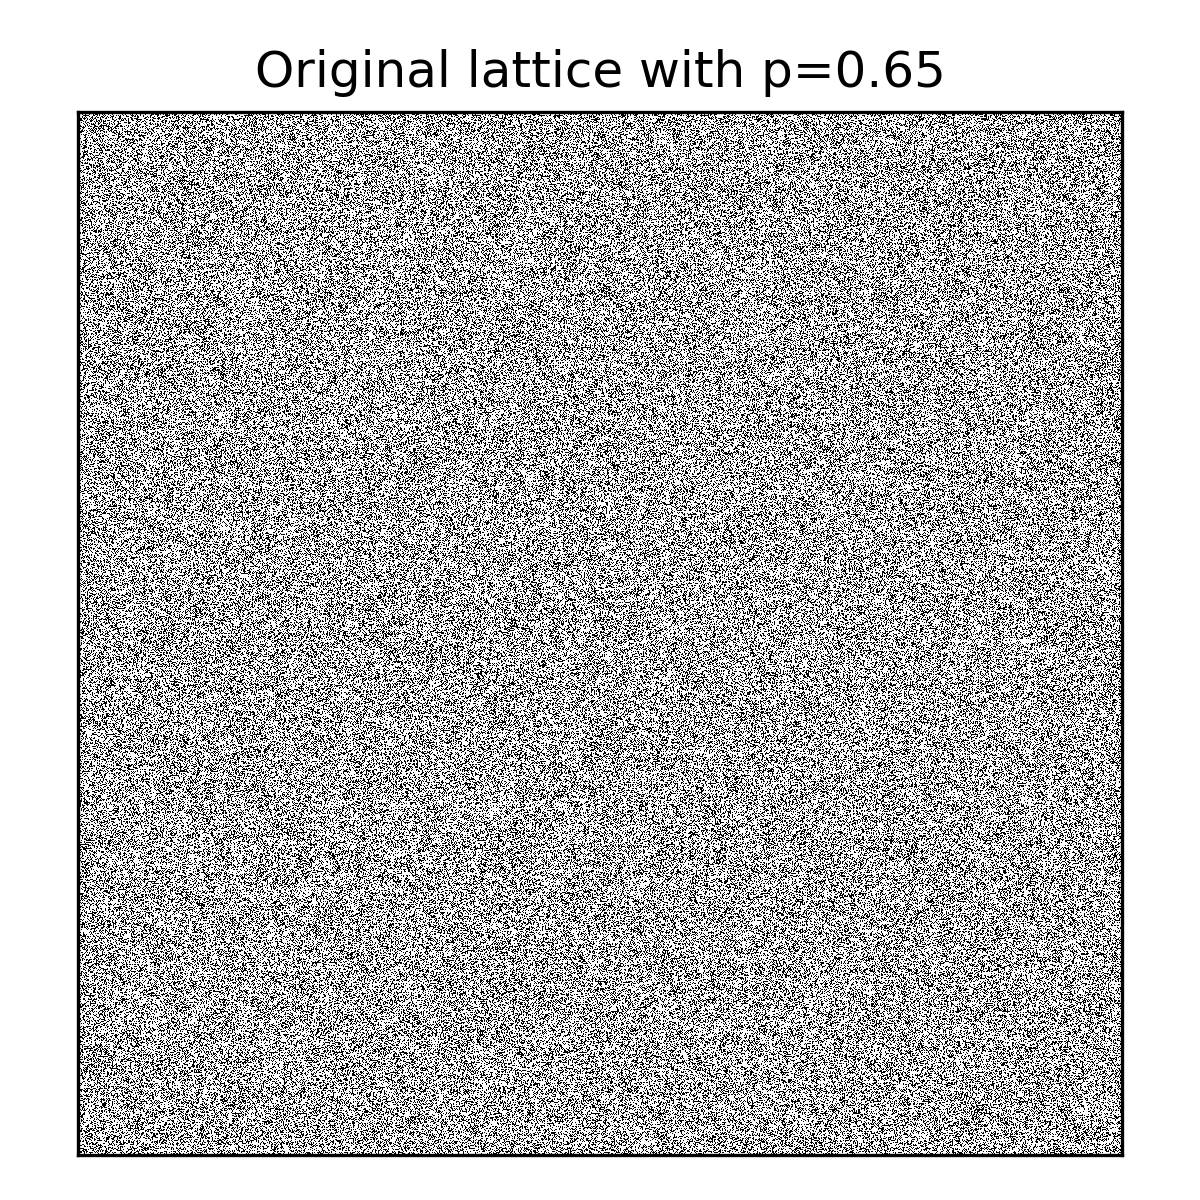
\includegraphics[width=0.3\textwidth]{images/Original lattice with p=0.65.png}
    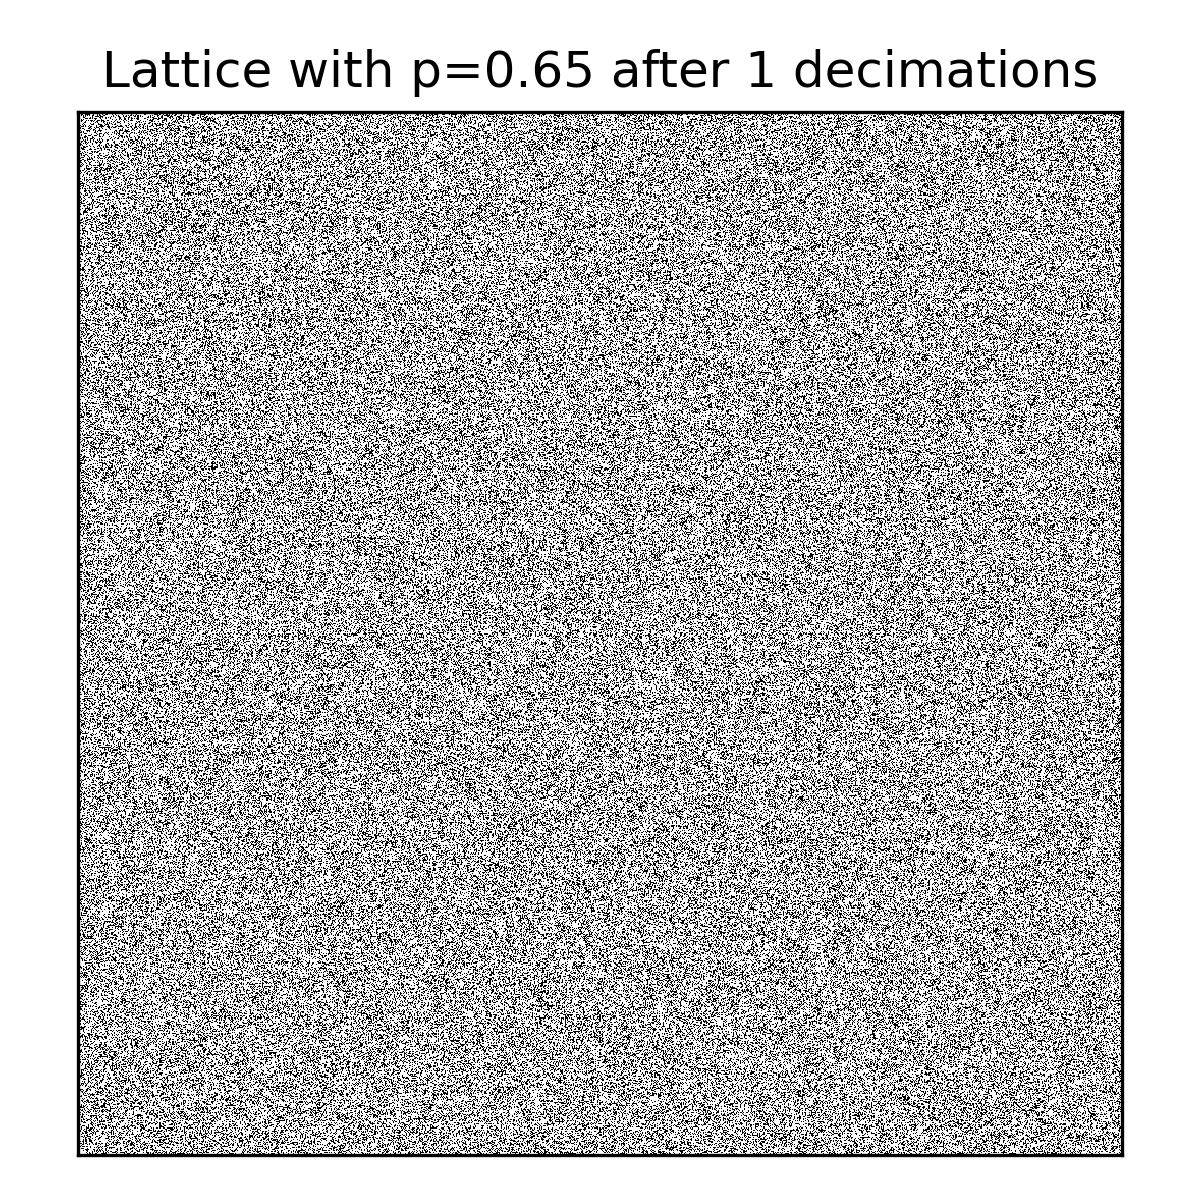
\includegraphics[width=0.3\textwidth]{images/Lattice with p=0.65 after 1 decimations.png}
    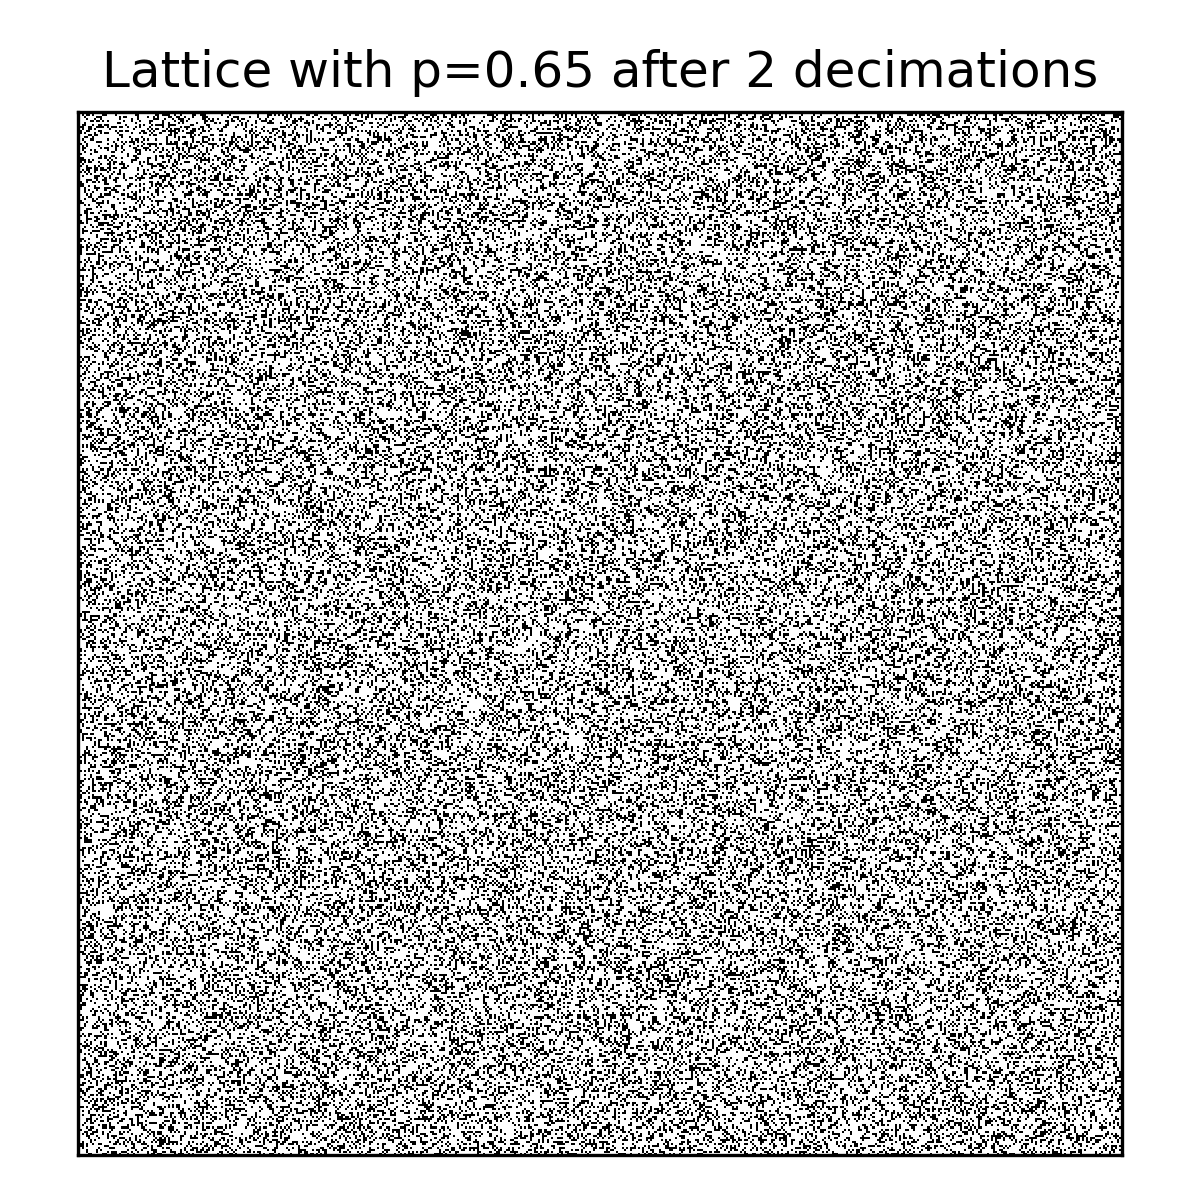
\includegraphics[width=0.3\textwidth]{images/Lattice with p=0.65 after 2 decimations.png}
    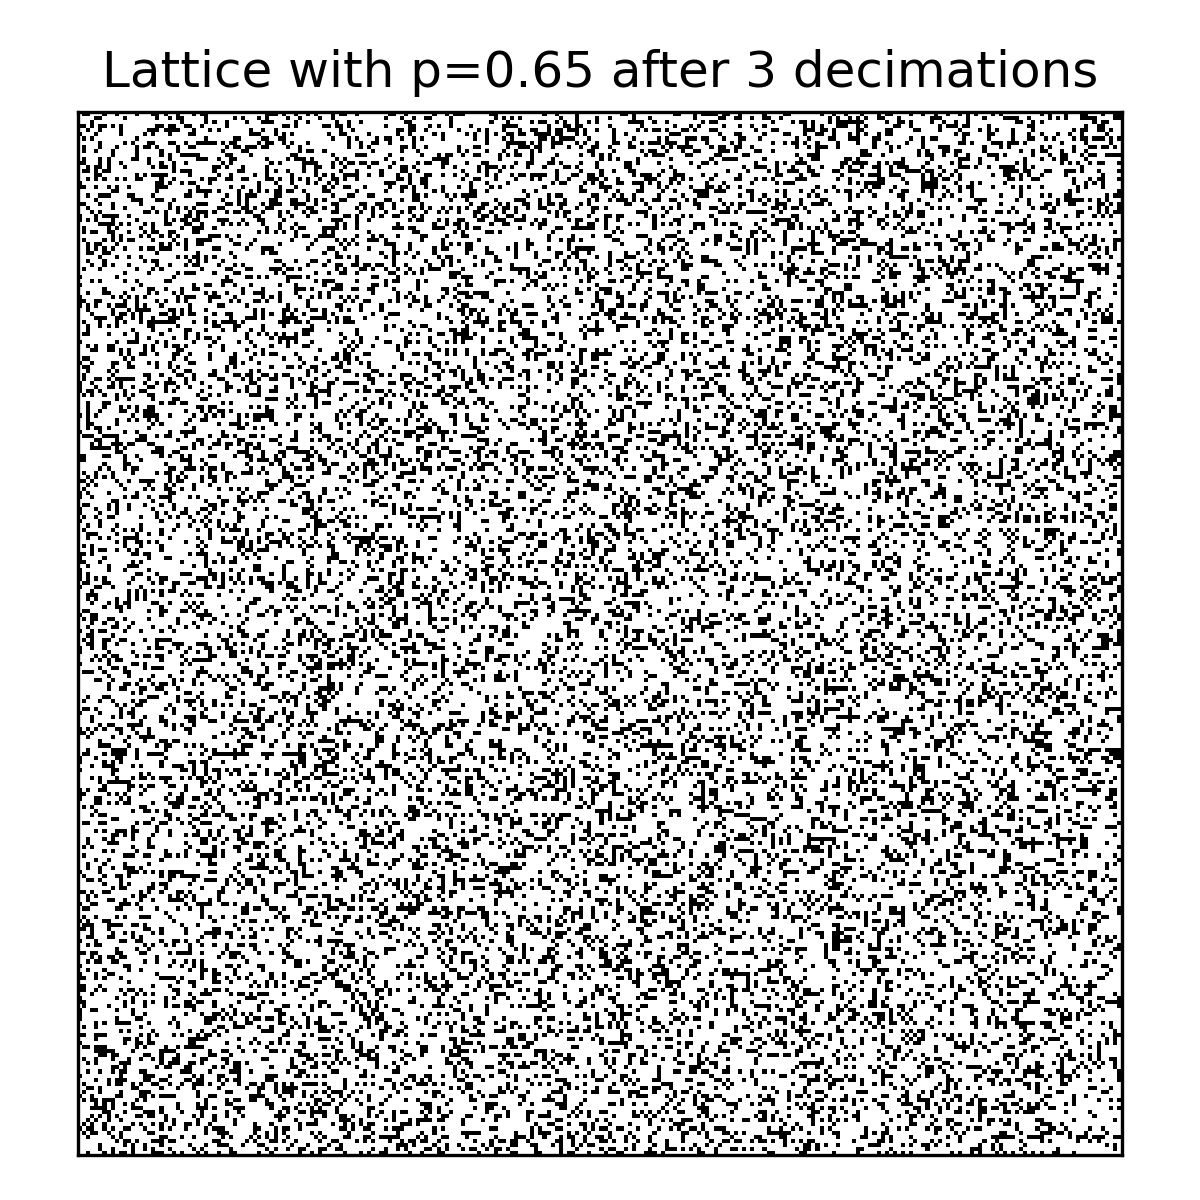
\includegraphics[width=0.3\textwidth]{images/Lattice with p=0.65 after 3 decimations.png}
    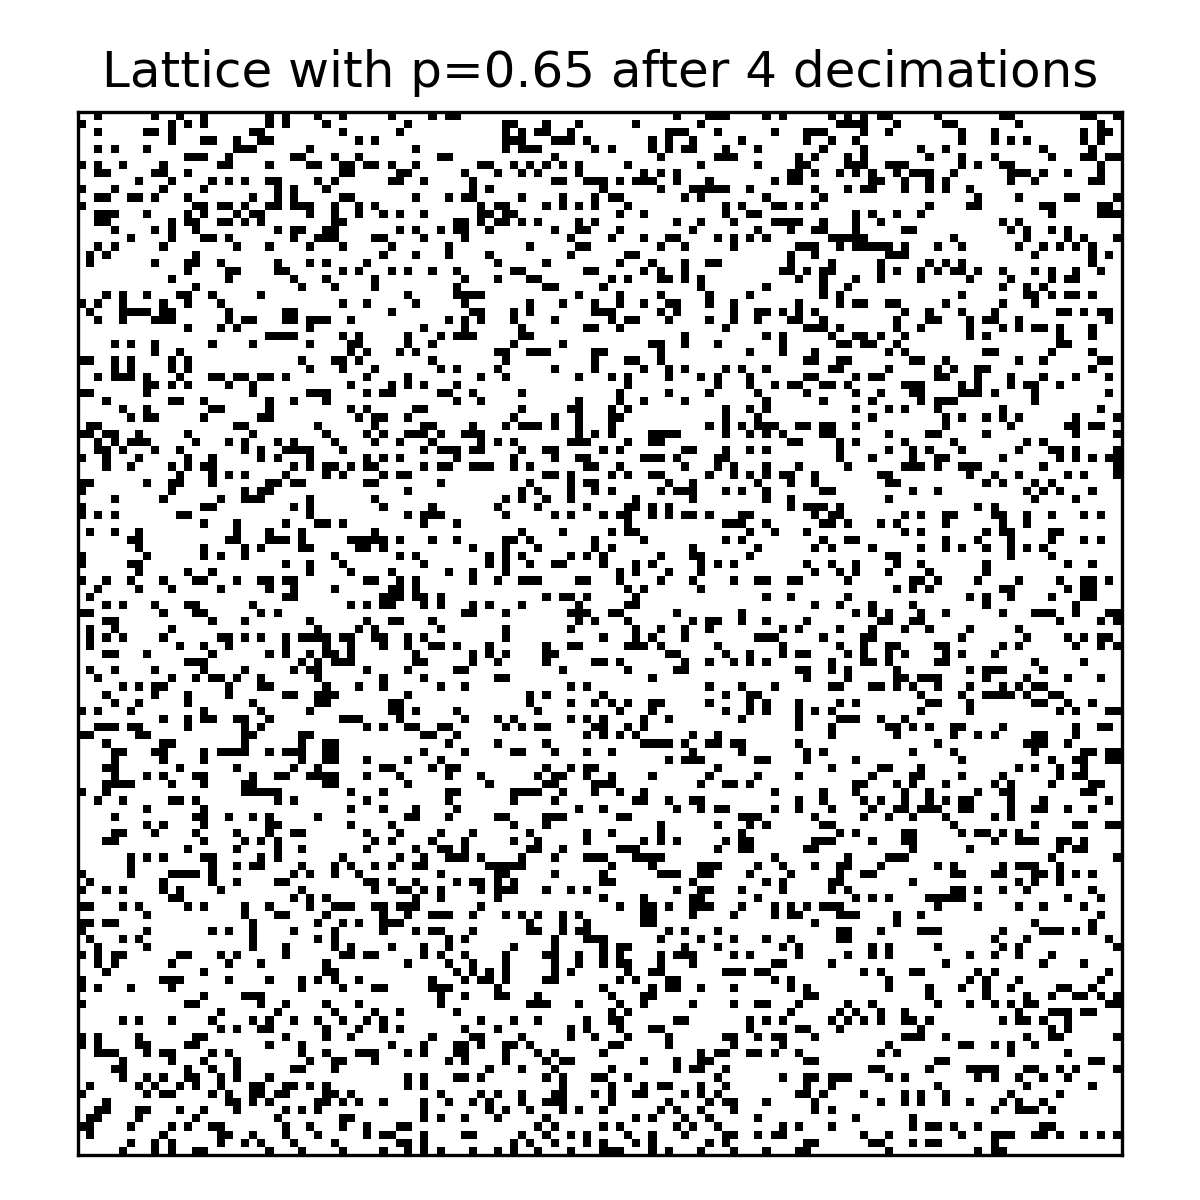
\includegraphics[width=0.3\textwidth]{images/Lattice with p=0.65 after 4 decimations.png}
    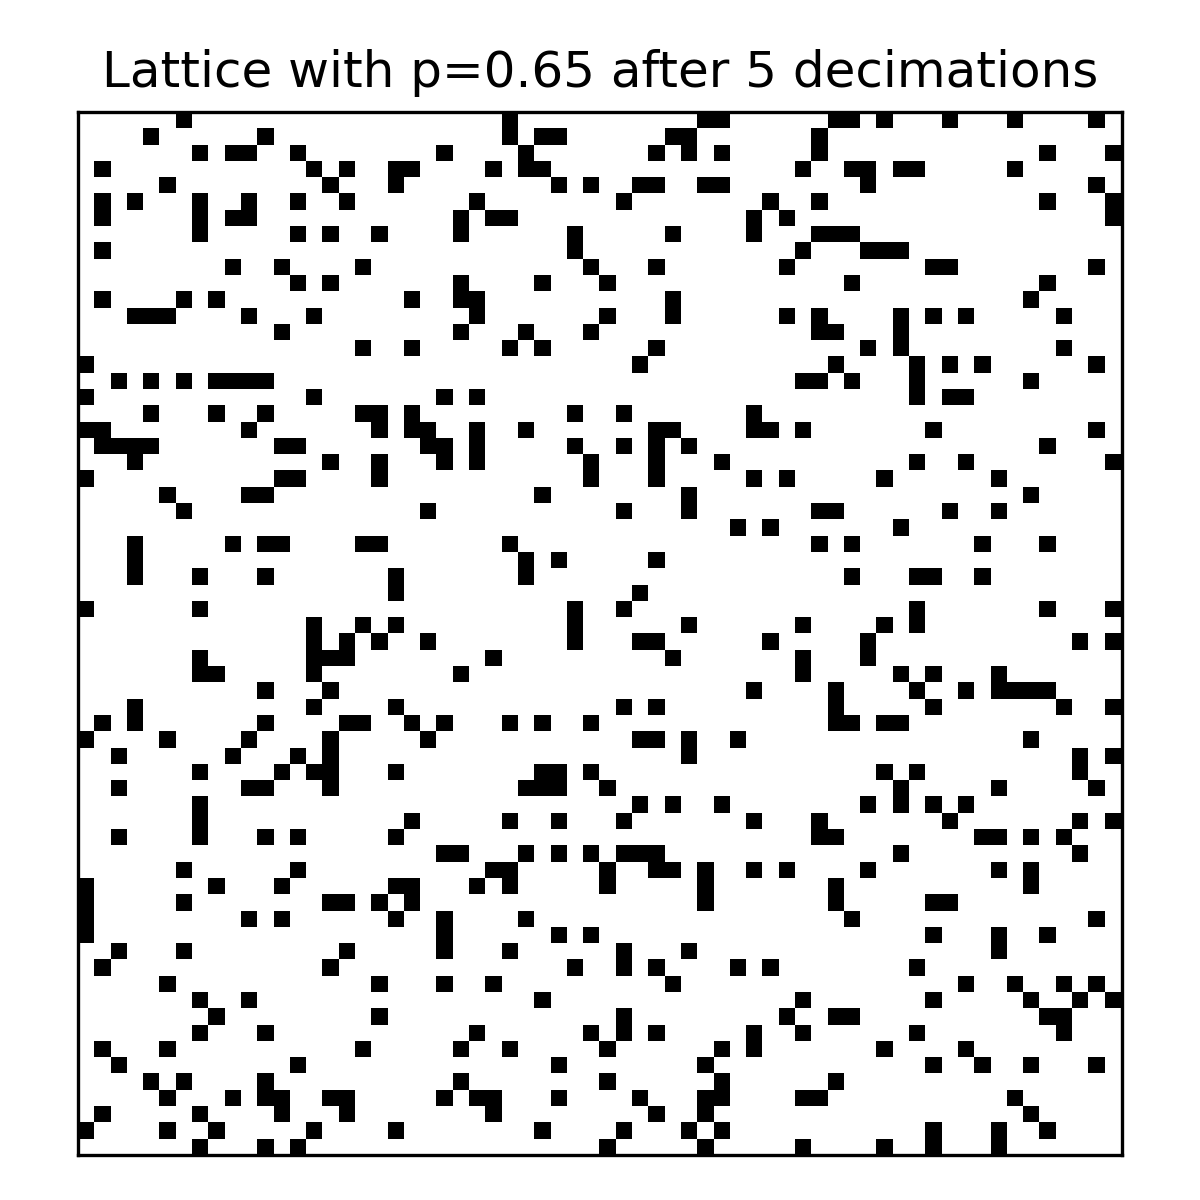
\includegraphics[width=0.3\textwidth]{images/Lattice with p=0.65 after 5 decimations.png}
    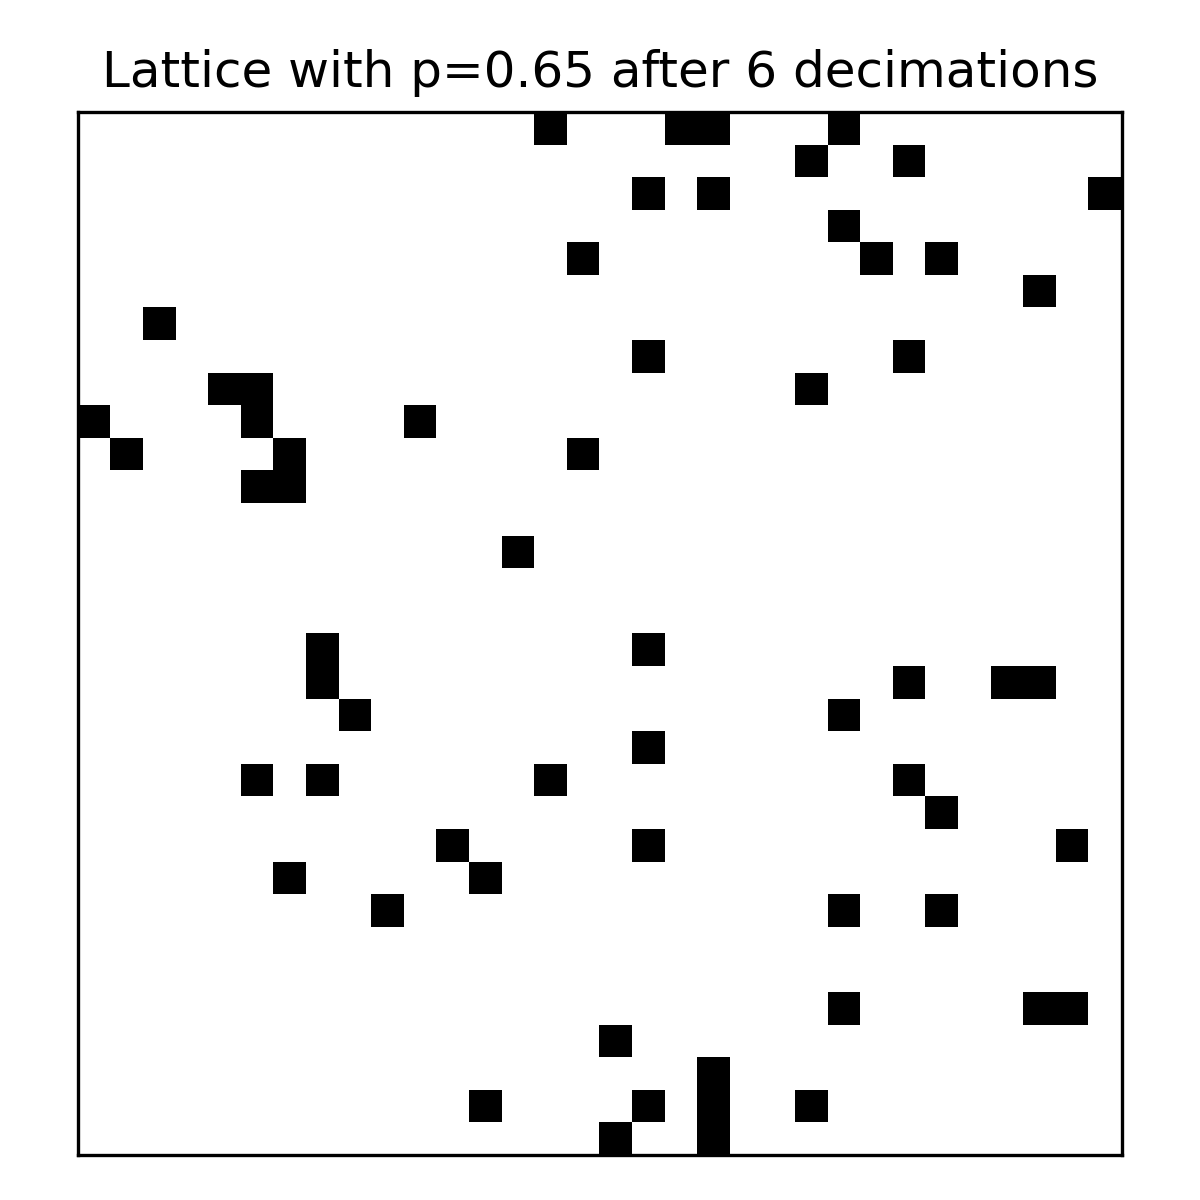
\includegraphics[width=0.3\textwidth]{images/Lattice with p=0.65 after 6 decimations.png}
    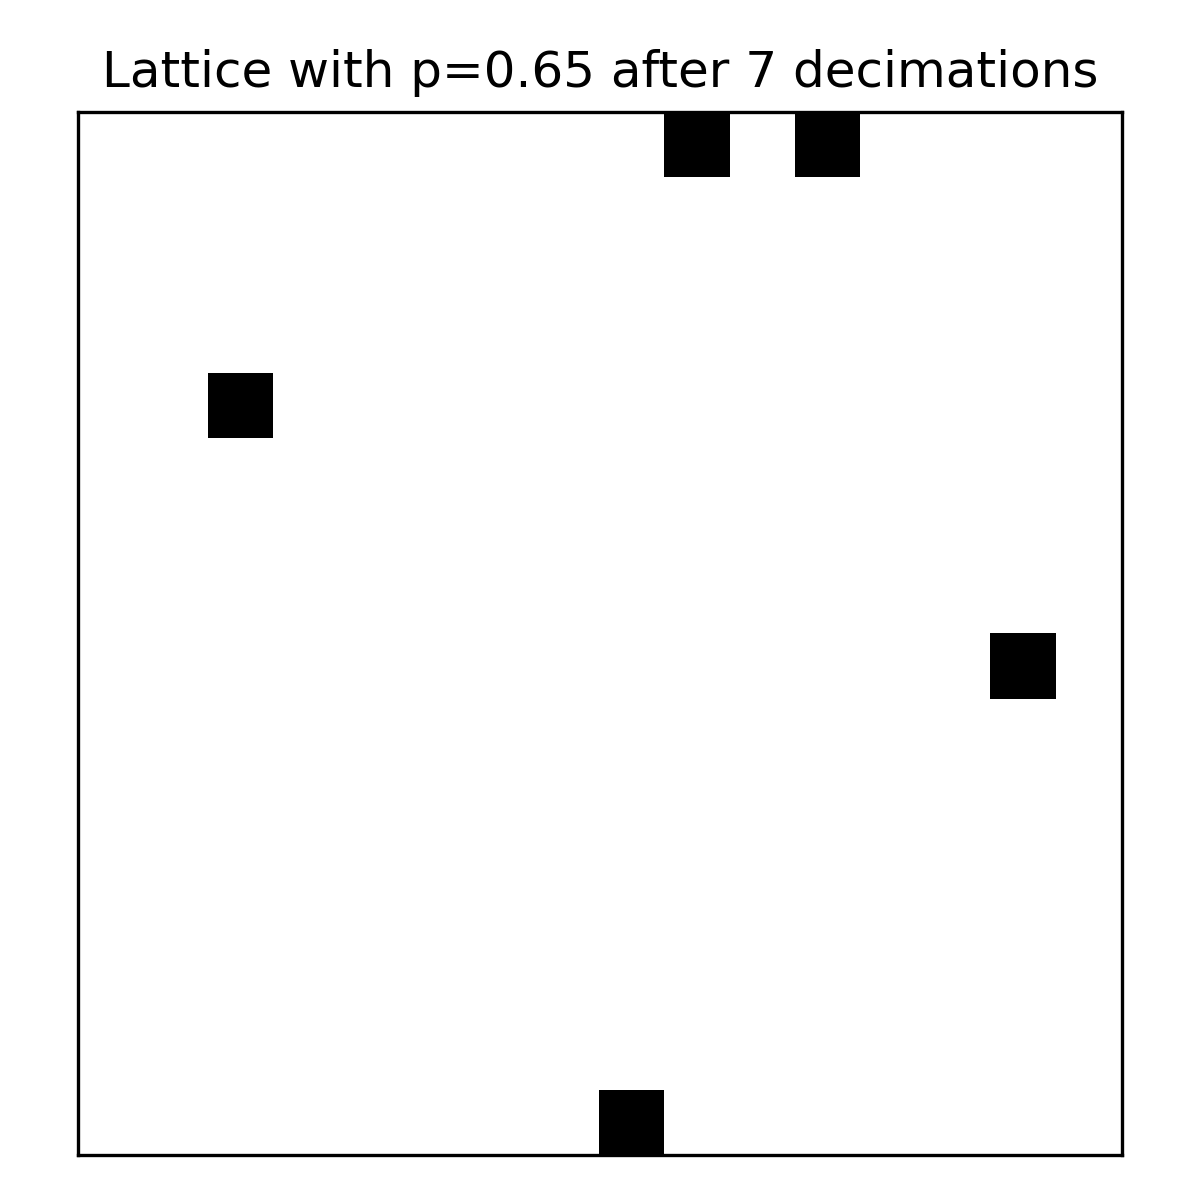
\includegraphics[width=0.3\textwidth]{images/Lattice with p=0.65 after 7 decimations.png}
    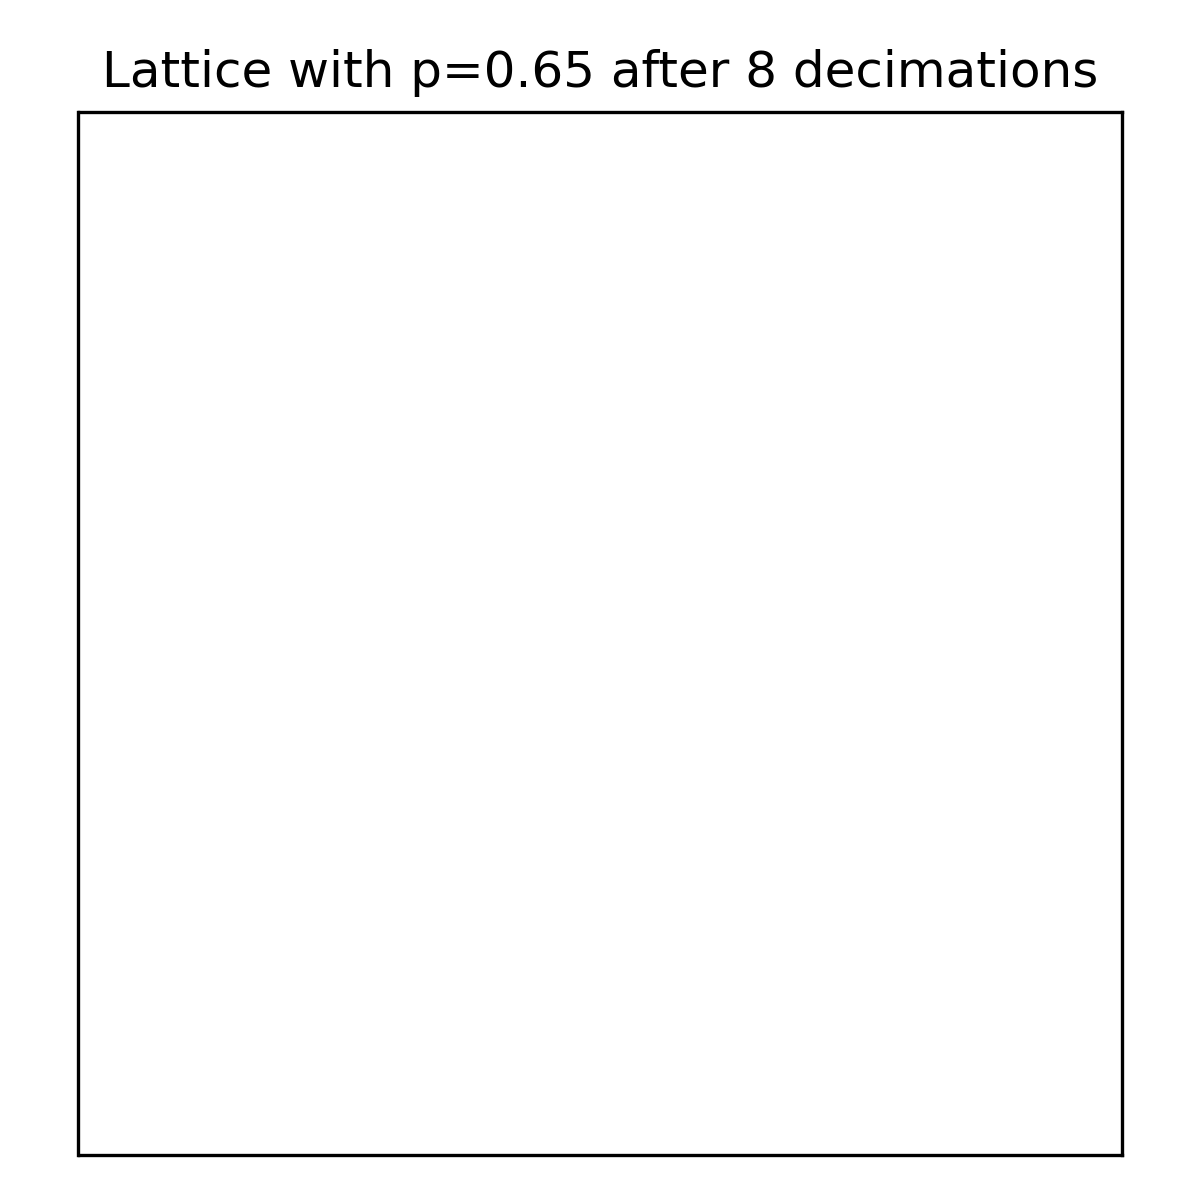
\includegraphics[width=0.3\textwidth]{images/Lattice with p=0.65 after 8 decimations.png}
    \caption{A lattice with $p=0.65$ in different stages of the coarse graining. Occupied cites are white.}
    \label{fig:lattices_65}
\end{figure}
\end{document}